%%%%%%%%%%%%%%%%%%%%%%%%%%%%%%%%%%%%%%%%%%%%%%%%%%%%%%%%%%%%%%%%%%%%%%%%%%%%%%%%
%%% Modelo para trabalhos monográficos (TCC, Dissertações, Teses, etc.) da
%%% Universidade Vila Velha (UVV) (https://www.uvv.br), utilizando a classe
%%% uvvTeX2.
%%%
%%% Para maiores informações, visite:
%%%    https://github.com/uvv-computacao/uvvtex2


%%%%%%%%%%%%%%%%%%%%%%%%%%%%%%%%%%%%%%%%%%%%%%%%%%%%%%%%%%%%%%%%%%%%%%%%%%%%%%%%
%%% Classe do documento
%%% As opções padronizadas abaixo são otimizadas para a apresentação monográfica
%%% na UVV: só altere se souber exatamente o que está fazendo.
\documentclass[
	% -- opções da classe memoir (utilizada pela abnTeX2) --
	12pt,				  % tamanho da fonte
	openright,			  % capítulos começam em página ímpar
	twoside,			  % impressão nos dois lados do papel
	a4paper,			  % tamanho do papel
	% -- opções da classe abnTeX2 (utilizada pela uvvTeX2) --
	%chapter=TITLE,		  % capítulos em letras maiúsculas
	%section=TITLE,		  % seções em letras maiúsculas
	%subsection=TITLE,	  % subseções em letras maiúsculas
	%subsubsection=TITLE,     % subsubseções em letras maiúsculas
	% -- opções do pacote babel --
	english,			% idioma adicional para hifenização
	french,				% idioma adicional para hifenização
	spanish,			% idioma adicional para hifenização
	brazil				% o último idioma é o principal do documento
	]{uvvtex2}


%%%%%%%%%%%%%%%%%%%%%%%%%%%%%%%%%%%%%%%%%%%%%%%%%%%%%%%%%%%%%%%%%%%%%%%%%%%%%%%%
%%% Dados da monografia
%%% Preencha conforme as instruções a seguir.

% Informe o título da monografia (lembre-se: um título objetivo e curto é melhor
% do que um título longo).
\titulo{Arquitetura em Nuvem com AWS: Uma Proposta Escalável, Segura e de Baixo Custo}

% Informe o(s) autor(es). Se houver mais de 1 autor, separar os autores com o
% comando " \and " (sem as aspas).
\autor{Igor Peli Resende}

% Informe o local no formato Cidade/UF (geralmente não é necessário alterar).
\local{Vila Velha/ES}

% Informe o ano.
\data{2025}

% Informe o nome do orientador (por extenso). Se for mulher, ajuste a
% qualificação que está entre colchetes.
\orientador[Orientador:]{Abrantes Araújo Silva Filho}

% Informe o nome do coorientador (por extenso). Se for mulher, ajuste a
% qualificação que está entre colchetes. Se não houver coorientador, comentar
% a linha.
%\coorientador[Coorientador:]{Nome do Coorientador}

% Informe a unidade ou o departamento de seu curso na UVV.
\unidadeuvv{Unidade de Tecnologia}

% Informe qual o seu curso na UVV.
\cursouvv{Graduação em Ciência da Computação}

% Informe que tipo de trabalho monográfico é este, com uma das seguintes opções:
%    Trabalho de Conclusão de Curso
%    Dissertação de Mestrado
%    Tese de Doutorado
\tipotrabalho{Trabalho de Conclusão de Curso}

% Nome oficial da UVV (evite alterar).
\nomeuvv{Universidade Vila Velha}

% Informe o preâmbulo da monografia (geralmente o tipo de trabalho, o objetivo,
% o nome da instituição e a área de concentração). Consulte seu orientador para
% instruções específicas se necessário, ou altere o modelo abaixo conforme
% suas necessidades (não retire os comandos "\imprimirunidadeuvv" e
% "\imprimirnomeuvv").
\preambulo{Trabalho Preliminar de Conclusão de Curso (TCC-1) apresentado à
\imprimirunidadeuvv\ da \imprimirnomeuvv, como requisito parcial para a
obtenção do grau de bacharel em Ciência da Computação.}

% Palavras-chave da monografia, em português. Essas palavras-chave serão
% incluídas automaticamente no resumo em português, e nas propriedades do
% arquivo PDF final gerado.
\palavraschave{Arquitetura em Nuvem, AWS, Escalabilidade, Profissionais Não Qualificados, Comparativo Nuvem vs On-Premises}

% Keywords (palavras-chave) da monografia, em inglês. Essas keywords serão
% incluídas automaticamente no abstract em inglês, e nas propriedades do arquivo
% PDF final gerado.
\keywords{Cloud Architecture, AWS, Scalability, Unqualified Professionals, Cloud vs On-Premises Comparison}

% Autor a ser utilizado na geração do código de Cutter da ficha catalográfica,
% no formato "Sobrenome, Nome". Atenção: se a monografia tiver dois autores,
% geralmente escreve-se aqui o nome do autor que está em primeiro lugar em
% ordem alfabética. Por exemplo: se os autores são "Fulano de Tal" e "Beltrano
% de Tal", escreveríamos aqui "Tal, Beltrano de".
\autorcutter{Resende, Igor}

% Código de cutter. Gere o código com alguma ferramente online (por exemplo:
% https://www.tabelacutter.com ou https://cuttersonline.com) e escreve o código
% aqui. Atenção: como nome do autor use "Sobrenome, Nome" e como complemento ou
% marca, use a primeira letra do título da monografia, em minúscula. Se você
% tiver dificuldade, peça auxílio à bibliotecária da UVV.
\cutter{R433a}

% Assuntos para a ficha catalográfica. É obrigatório incluir pelo menos 1
% assunto (até o total de 5). Colocar ponto após o número do assunto e após o
% próprio assunto. Comentar os que, por acaso, não forem utilizados. Se você
% tiver dificuldade, peça auxílio à bibliotecária da UVV.
\assunto{%
1. Computação em nuvem.
2. Amazon Web Services (AWS).
3. Infraestrutura como código.
4. Arquitetura escalável.
5. Comparativo entre nuvem e on-premises.
I. Resende, Igor.                 % Seu nome como autor
II. Araújo, Abrantes.             % Substitua pelo nome do orientador
III. Universidade Vila Velha.     % Nome da instituição
IV. Arquitetura em nuvem com AWS. % Título resumido ou completo do TCC
}

% NÃO ALTERE AQUI:
%%%%%%%%%%%%%%%%%%%%%%%%%%%%%%%%%%%%%%%%%%%%%%%%%%%%%%%%%%%%%%%%%%%%%%%%%%%%%%%%
% uvv.tex
%
% Arquivo de configuração de packages para uso com a classe uvvTeX2, para a
% formatação de trabalhos acadêmicos na Universidade Vila Velha (UVV)
% (https://www.uvv.br).
%
% Para maiores informações, visite:
%    https://github.com/uvv-computacao/uvvtex2
%
% NÃO ALTERE NADA AQUI!
%%%%%%%%%%%%%%%%%%%%%%%%%%%%%%%%%%%%%%%%%%%%%%%%%%%%%%%%%%%%%%%%%%%%%%%%%%%%%%%%

% Imprime corretamente o nome oficial, a unidade e o curso:
\instituicao{%
  \imprimirnomeuvv
  \par
  \imprimirunidadeuvv
  \par
  \imprimircursouvv
}




%%%%%%%%%%%%%%%%%%%%%%%%%%%%%%%%%%%%%%%%%%%%%%%%%%%%%%%%%%%%%%%%%%%%%%%%%%%%%%%%
%%% Preâmbulo com a inclusão de todos os packages necessários
%%% Não altere!
%%%%%%%%%%%%%%%%%%%%%%%%%%%%%%%%%%%%%%%%%%%%%%%%%%%%%%%%%%%%%%%%%%%%%%%%%%%%%%%%
% preambulo.tex
%
% Arquivo de chamada de todos os outros arquivos de configurações de packages
% para uso com a classe uvvTeX2, para a formatação de trabalhos acadêmicos na
% Universidade Vila Velha (UVV) (https://www.uvv.br).
%
% Para maiores informações, visite:
%    https://github.com/abrantesasf/uvvtex2
%
% NÃO ALTERE NADA AQUI!
%%%%%%%%%%%%%%%%%%%%%%%%%%%%%%%%%%%%%%%%%%%%%%%%%%%%%%%%%%%%%%%%%%%%%%%%%%%%%%%%


%%%%%%%%%%%%%%%%%%%%%%%%%%%%%%%%%%%%%%%%%%%%%%%%%%%%%%%%%%%%%%%%%%%%%%%%%%%%%%%%
%%% Estruturas de controle:
%%%%%%%%%%%%%%%%%%%%%%%%%%%%%%%%%%%%%%%%%%%%%%%%%%%%%%%%%%%%%%%%%%%%%%%%%%%%%%%%
% controles.tex
%
% Arquivo de configuração de packages para uso com a classe uvvTeX2, para a
% formatação de trabalhos acadêmicos na Universidade Vila Velha (UVV)
% (https://www.uvv.br).
%
% Para maiores informações, visite:
%    https://github.com/uvv-computacao/uvvtex2
%
% NÃO ALTERE NADA AQUI!
%%%%%%%%%%%%%%%%%%%%%%%%%%%%%%%%%%%%%%%%%%%%%%%%%%%%%%%%%%%%%%%%%%%%%%%%%%%%%%%%

% Carrega pacotes iniciais necessários para estrutura de controle e para a
% criação e o parse de novos comandos
%\usepackage{ifthen}     % já carregado pela classe abntex2
\usepackage{xparse}
\usepackage{ifxetex}



%%%%%%%%%%%%%%%%%%%%%%%%%%%%%%%%%%%%%%%%%%%%%%%%%%%%%%%%%%%%%%%%%%%%%%%%%%%%%%%%
%%% Compilação condicional em PDF:
%%%%%%%%%%%%%%%%%%%%%%%%%%%%%%%%%%%%%%%%%%%%%%%%%%%%%%%%%%%%%%%%%%%%%%%%%%%%%%%%
% pdf.tex
%
% Arquivo de configuração de packages para uso com a classe uvvTeX2, para a
% formatação de trabalhos acadêmicos na Universidade Vila Velha (UVV)
% (https://www.uvv.br).
%
% Para maiores informações, visite:
%    https://github.com/uvv-computacao/uvvtex2
%
% NÃO ALTERE NADA AQUI!
%%%%%%%%%%%%%%%%%%%%%%%%%%%%%%%%%%%%%%%%%%%%%%%%%%%%%%%%%%%%%%%%%%%%%%%%%%%%%%%%

% Pacotes para compilação condicional em PDF:
\ifxetex
\else
   \usepackage{ifpdf}
\fi



%%%%%%%%%%%%%%%%%%%%%%%%%%%%%%%%%%%%%%%%%%%%%%%%%%%%%%%%%%%%%%%%%%%%%%%%%%%%%%%%
%%% Configurações de layout da página:
%%%%%%%%%%%%%%%%%%%%%%%%%%%%%%%%%%%%%%%%%%%%%%%%%%%%%%%%%%%%%%%%%%%%%%%%%%%%%%%%
% layout.tex
%
% Arquivo de configuração de packages para uso com a classe uvvTeX2, para a
% formatação de trabalhos acadêmicos na Universidade Vila Velha (UVV)
% (https://www.uvv.br).
%
% Para maiores informações, visite:
%    https://github.com/uvv-computacao/uvvtex2
%
% NÃO ALTERE NADA AQUI!
%%%%%%%%%%%%%%%%%%%%%%%%%%%%%%%%%%%%%%%%%%%%%%%%%%%%%%%%%%%%%%%%%%%%%%%%%%%%%%%%

% Posiciona figuras e tabelas no topo da página quando adicionadas sozinhas
% em um página em branco. Ver https://github.com/abntex/abntex2/issues/170
\makeatletter
\setlength{\@fptop}{5pt}   % Set distance from top of page to first float
\makeatother

% O tamanho do parágrafo é dado por:
\setlength{\parindent}{1.3cm}

% Controle do espaçamento entre um parágrafo e outro:
\setlength{\parskip}{0.2cm}  % tente também \onelineskip

% Para melhorias de justificação
\usepackage{microtype}

% Para contar págians
\usepackage{lastpage}



%%%%%%%%%%%%%%%%%%%%%%%%%%%%%%%%%%%%%%%%%%%%%%%%%%%%%%%%%%%%%%%%%%%%%%%%%%%%%%%%
%%% Configurações para autores:
%%%%%%%%%%%%%%%%%%%%%%%%%%%%%%%%%%%%%%%%%%%%%%%%%%%%%%%%%%%%%%%%%%%%%%%%%%%%%%%%
% autores.tex
%
% Arquivo de configuração de packages para uso com a classe uvvTeX2, para a
% formatação de trabalhos acadêmicos na Universidade Vila Velha (UVV)
% (https://www.uvv.br).
%
% Para maiores informações, visite:
%    https://github.com/uvv-computacao/uvvtex2
%
% NÃO ALTERE NADA AQUI!
%%%%%%%%%%%%%%%%%%%%%%%%%%%%%%%%%%%%%%%%%%%%%%%%%%%%%%%%%%%%%%%%%%%%%%%%%%%%%%%%

% Ajustes para os autores e afiliações, em artigos
\makeatletter
\@ifclassloaded{article}{
\usepackage{authblk}
}{}
\makeatother



%%%%%%%%%%%%%%%%%%%%%%%%%%%%%%%%%%%%%%%%%%%%%%%%%%%%%%%%%%%%%%%%%%%%%%%%%%%%%%%%
%%% Configuração para as fontes do documento:
%%% Se você quiser usar fontes próprias ou do sistema, precisará ajustar as
%%% configurações no arquivo "utils/fontes.tex".
%%% ATENÇÃO: por padrão eu utilizo XeLaTeX com fontes proprietárias projetadas
%%% por Matthew Butterick, adquiridas em https://mbtype.com, que não podem ser
%%% distribuídas devido à licença de utilização. Se você usar XeLaTeX, você
%%% DEVERÁ OBRIGATORIAMENTE ajustar as fontes no arquivo "utils/fontes.tex".
%%%%%%%%%%%%%%%%%%%%%%%%%%%%%%%%%%%%%%%%%%%%%%%%%%%%%%%%%%%%%%%%%%%%%%%%%%%%%%%%
% fontes.tex
%
% Arquivo de configuração de packages para uso com a classe uvvTeX2, para a
% formatação de trabalhos acadêmicos na Universidade Vila Velha (UVV)
% (https://www.uvv.br).
%
% Para maiores informações, visite:
%    https://github.com/uvv-computacao/uvvtex2
%
% Você deve informar abaixo quais são as fontes que você quer usar na sua
% monografia, se utilizar o XeLaTeX para a compilação. Se usar o pdfLaTeX a
% monografia será impressa com as fontes padronizadas do TeX.
%%%%%%%%%%%%%%%%%%%%%%%%%%%%%%%%%%%%%%%%%%%%%%%%%%%%%%%%%%%%%%%%%%%%%%%%%%%%%%%%

% Configurações de encodings e fontes:
\ifxetex
   % Se usar XeLaTeX, usa fontes específicas:
   \usepackage[tuenc,no-math]{fontspec}
   \setmainfont{equity-text-a-regular.otf}[
      Path           = /home/abrantesasf/.local/share/fonts/ ,
      BoldFont       = equity-text-a-bold.otf                ,
      ItalicFont     = equity-text-a-italic.otf              ,
      BoldItalicFont = equity-text-a-bold-italic.otf]
   \setsansfont{equity-text-b-regular.otf}[
      Path           = /home/abrantesasf/.local/share/fonts/ ,
      BoldFont       = equity-text-b-bold.otf                ,
      ItalicFont     = equity-text-b-italic.otf              ,
      BoldItalicFont = equity-text-b-bold-italic.otf]
   \setmonofont{triplicate-t4-regular.otf}[
      Path           = /home/abrantesasf/.local/share/fonts/ ,
      BoldFont       = triplicate-t4-bold.otf                ,
      ItalicFont     = triplicate-t4-italic.otf              ,
      BoldItalicFont = triplicate-t4-bold-italic.otf]
   \usepackage{fontawesome5}
\else
   % Se não for XeLaTeX, vai com as normais mesmo:
   \usepackage[T1]{fontenc}
   \usepackage[utf8]{inputenc}
   \usepackage{lmodern}
   % Altera a fonte padrão do documento (nem todas funcionam em modo math):
   %   phv = Helvetica
   %   ptm = Times
   %   ppl = Palatino
   %   pbk = bookman
   %   pag = AdobeAvantGarde
   %   pnc = Adobe NewCenturySchoolBook
   %\renewcommand{\familydefault}{ppl}
\fi



%%%%%%%%%%%%%%%%%%%%%%%%%%%%%%%%%%%%%%%%%%%%%%%%%%%%%%%%%%%%%%%%%%%%%%%%%%%%%%%%
%%% Sumário:
%%%%%%%%%%%%%%%%%%%%%%%%%%%%%%%%%%%%%%%%%%%%%%%%%%%%%%%%%%%%%%%%%%%%%%%%%%%%%%%%
% toc.tex
%
% Arquivo de configuração de packages para uso com a classe uvvTeX2, para a
% formatação de trabalhos acadêmicos na Universidade Vila Velha (UVV)
% (https://www.uvv.br).
%
% Para maiores informações, visite:
%    https://github.com/uvv-computacao/uvvtex2
%
% NÃO ALTERE NADA AQUI!
%%%%%%%%%%%%%%%%%%%%%%%%%%%%%%%%%%%%%%%%%%%%%%%%%%%%%%%%%%%%%%%%%%%%%%%%%%%%%%%%

% Ajustes de sumário:
\makeatletter
\@ifclassloaded{article}{
   \usepackage[nottoc]{tocbibind}
   %\usepackage{tocbibind}
}{}
\@ifclassloaded{book}{
   \usepackage{tocbibind}
}{}
\makeatother



%%%%%%%%%%%%%%%%%%%%%%%%%%%%%%%%%%%%%%%%%%%%%%%%%%%%%%%%%%%%%%%%%%%%%%%%%%%%%%%%
%%% Matemática:
%%%%%%%%%%%%%%%%%%%%%%%%%%%%%%%%%%%%%%%%%%%%%%%%%%%%%%%%%%%%%%%%%%%%%%%%%%%%%%%%
% matematica.tex
%
% Arquivo de configuração de packages para uso com a classe uvvTeX2, para a
% formatação de trabalhos acadêmicos na Universidade Vila Velha (UVV)
% (https://www.uvv.br).
%
% Para maiores informações, visite:
%    https://github.com/uvv-computacao/uvvtex2
%
% Geralmente não é necessário alterar nada aqui!
%%%%%%%%%%%%%%%%%%%%%%%%%%%%%%%%%%%%%%%%%%%%%%%%%%%%%%%%%%%%%%%%%%%%%%%%%%%%%%%%

% Carrega bibliotecas e símbolos matemáticos, fontes adicionais e configura
% algumas outras opções
\usepackage{amsmath}
\usepackage{amssymb}
\usepackage{amsthm}
\usepackage{amsfonts}
\usepackage{mathrsfs}
\usepackage{proof}
\usepackage{siunitx}
  \sisetup{group-separator = {\,}}
  \sisetup{group-digits = {integer}}
  \sisetup{output-decimal-marker = {,}}
  \sisetup{separate-uncertainty}
  \sisetup{multi-part-units = single}
  \sisetup{binary-units = true}
\usepackage{bm}
\usepackage{cancel}

% Altera separador decimal via comando, se necessário (prefira o siunitx):
%\mathchardef\period=\mathcode`.
%\DeclareMathSymbol{.}{\mathord}{letters}{"3B}

\usepackage{esvect}
\usepackage{mathtools}

% Definições para teoremas, etc.
\theoremstyle{definition}
\newtheorem{definicao}{Definição}[chapter]
\newtheorem{conjecture}{Conjectura}[chapter]
\newtheorem{teorema}{Teorema}[chapter]
\newtheorem{lemma}{Lema}[chapter]
\newtheorem{corolario}{Corolário}[chapter]



%%%%%%%%%%%%%%%%%%%%%%%%%%%%%%%%%%%%%%%%%%%%%%%%%%%%%%%%%%%%%%%%%%%%%%%%%%%%%%%%
%%% Referências bibliográficas:
%%%%%%%%%%%%%%%%%%%%%%%%%%%%%%%%%%%%%%%%%%%%%%%%%%%%%%%%%%%%%%%%%%%%%%%%%%%%%%%%
% bibliografia.tex
%
% Arquivo de configuração de packages para uso com a classe uvvTeX2, para a
% formatação de trabalhos acadêmicos na Universidade Vila Velha (UVV)
% (https://www.uvv.br).
%
% Para maiores informações, visite:
%    https://github.com/uvv-computacao/uvvtex2
%
% NÃO ALTERE NADA AQUI!
%%%%%%%%%%%%%%%%%%%%%%%%%%%%%%%%%%%%%%%%%%%%%%%%%%%%%%%%%%%%%%%%%%%%%%%%%%%%%%%%

% Referências bibliográficas
\usepackage[brazilian,hyperpageref]{backref} % Páginas onde foi citado
\usepackage[alf]{abntex2cite}	             % Citações padrão ABNT

% Configurações do pacote backref:
\renewcommand{\backrefpagesname}{Citado na(s) página(s):~}
\renewcommand{\backref}{}
\renewcommand*{\backrefalt}[4]{
	\ifcase #1 %
		Nenhuma citação no texto.%
	\or
		Citado na página #2.%
	\else
		Citado #1 vezes, nas páginas #2.%
	\fi}%



%%%%%%%%%%%%%%%%%%%%%%%%%%%%%%%%%%%%%%%%%%%%%%%%%%%%%%%%%%%%%%%%%%%%%%%%%%%%%%%%
%%% Cores:
%%%%%%%%%%%%%%%%%%%%%%%%%%%%%%%%%%%%%%%%%%%%%%%%%%%%%%%%%%%%%%%%%%%%%%%%%%%%%%%%
% cores.tex
%
% Arquivo de configuração de packages para uso com a classe uvvTeX2, para a
% formatação de trabalhos acadêmicos na Universidade Vila Velha (UVV)
% (https://www.uvv.br).
%
% Para maiores informações, visite:
%    https://github.com/uvv-computacao/uvvtex2
%
% NÃO ALTERE NADA AQUI!
%%%%%%%%%%%%%%%%%%%%%%%%%%%%%%%%%%%%%%%%%%%%%%%%%%%%%%%%%%%%%%%%%%%%%%%%%%%%%%%%

% Ativa suporte extendido a cores
% Opções comuns:
%    usenames (16)
%    dvipsnames (64)
%    svgnames (150)
%    x11names (300)
\makeatletter
\@ifclassloaded{beamer}{
   % Beamer sem opções
  \usepackage{xcolor} 
}{
   % Resto opção svgnames
  \usepackage[svgnames, table]{xcolor}
}
\makeatother



%%%%%%%%%%%%%%%%%%%%%%%%%%%%%%%%%%%%%%%%%%%%%%%%%%%%%%%%%%%%%%%%%%%%%%%%%%%%%%%%
%%% Computação:
%%%%%%%%%%%%%%%%%%%%%%%%%%%%%%%%%%%%%%%%%%%%%%%%%%%%%%%%%%%%%%%%%%%%%%%%%%%%%%%%
% computacao.tex
%
% Arquivo de configuração de packages para uso com a classe uvvTeX2, para a
% formatação de trabalhos acadêmicos na Universidade Vila Velha (UVV)
% (https://www.uvv.br).
%
% Para maiores informações, visite:
%    https://github.com/uvv-computacao/uvvtex2
%
% NÃO ALTERE NADA AQUI!
%%%%%%%%%%%%%%%%%%%%%%%%%%%%%%%%%%%%%%%%%%%%%%%%%%%%%%%%%%%%%%%%%%%%%%%%%%%%%%%%

% Carrega packages relacionados à computação
\usepackage{algorithm2e}
\usepackage{algorithmicx}
\usepackage{algpseudocode}
\usepackage{listings}
  \lstset{literate=
    {á}{{\'a}}1 {é}{{\'e}}1 {í}{{\'i}}1 {ó}{{\'o}}1 {ú}{{\'u}}1
    {Á}{{\'A}}1 {É}{{\'E}}1 {Í}{{\'I}}1 {Ó}{{\'O}}1 {Ú}{{\'U}}1
    {à}{{\`a}}1 {è}{{\`e}}1 {ì}{{\`i}}1 {ò}{{\`o}}1 {ù}{{\`u}}1
    {À}{{\`A}}1 {È}{{\'E}}1 {Ì}{{\`I}}1 {Ò}{{\`O}}1 {Ù}{{\`U}}1
    {ä}{{\"a}}1 {ë}{{\"e}}1 {ï}{{\"i}}1 {ö}{{\"o}}1 {ü}{{\"u}}1
    {Ä}{{\"A}}1 {Ë}{{\"E}}1 {Ï}{{\"I}}1 {Ö}{{\"O}}1 {Ü}{{\"U}}1
    {â}{{\^a}}1 {ê}{{\^e}}1 {î}{{\^i}}1 {ô}{{\^o}}1 {û}{{\^u}}1
    {Â}{{\^A}}1 {Ê}{{\^E}}1 {Î}{{\^I}}1 {Ô}{{\^O}}1 {Û}{{\^U}}1
    {œ}{{\oe}}1 {Œ}{{\OE}}1 {æ}{{\ae}}1 {Æ}{{\AE}}1 {ß}{{\ss}}1
    {ű}{{\H{u}}}1 {Ű}{{\H{U}}}1 {ő}{{\H{o}}}1 {Ő}{{\H{O}}}1
    {ç}{{\c c}}1 {Ç}{{\c C}}1 {ø}{{\o}}1 {å}{{\r a}}1 {Å}{{\r A}}1
    {€}{{\euro}}1 {£}{{\pounds}}1 {«}{{\guillemotleft}}1
    {»}{{\guillemotright}}1 {ñ}{{\~n}}1 {Ñ}{{\~N}}1 {¿}{{?`}}1
  }
\definecolor{mGreen}{rgb}{0,0.6,0}
\definecolor{mGray}{rgb}{0.5,0.5,0.5}
\definecolor{mPurple}{rgb}{0.58,0,0.82}
\definecolor{backgroundColour}{rgb}{0.95,0.95,0.92}
\lstdefinestyle{CStyle}{
    backgroundcolor=\color{backgroundColour},   
    commentstyle=\color{green}\ttfamily,
    keywordstyle=\color{blue}\ttfamily,
    numberstyle=\tiny\color{mGray},
    stringstyle=\color{red}\ttfamily,
    basicstyle=\ttfamily,
    morecomment=[l][\color{magenta}]{\#},
    breakatwhitespace=false,         
    breaklines=true,                 
    captionpos=b,                    
    keepspaces=true,                 
    numbers=left,                    
    numbersep=5pt,                  
    showspaces=false,                
    showstringspaces=false,
    showtabs=false,                  
    tabsize=4,
    language=C
}


%%%%%%%%%%%%%%%%%%%%%%%%%%%%%%%%%%%%%%%%%%%%%%%%%%%%%%%%%%%%%%%%%%%%%%%%%%%%%%%%
%%% Gráficos:
%%%%%%%%%%%%%%%%%%%%%%%%%%%%%%%%%%%%%%%%%%%%%%%%%%%%%%%%%%%%%%%%%%%%%%%%%%%%%%%%
% graficos.tex
%
% Arquivo de configuração de packages para uso com a classe uvvTeX2, para a
% formatação de trabalhos acadêmicos na Universidade Vila Velha (UVV)
% (https://www.uvv.br).
%
% Para maiores informações, visite:
%    https://github.com/uvv-computacao/uvvtex2
%
% NÃO ALTERE NADA AQUI!
%%%%%%%%%%%%%%%%%%%%%%%%%%%%%%%%%%%%%%%%%%%%%%%%%%%%%%%%%%%%%%%%%%%%%%%%%%%%%%%%

% Suporte à importação de gráficos externos
\makeatletter
\@ifclassloaded{beamer}{
   \usepackage{graphicx}
}{
   \ifxetex
      \usepackage{graphicx}
   \else
      \ifpdf
         \usepackage[pdftex]{graphicx}
      \else
         \usepackage[dvips]{graphicx}
      \fi
   \fi
}
\makeatother


% Suporte à criação de gráficos proceduralmente no LaTeX:
\usepackage{tikz}
\usetikzlibrary{arrows,automata,backgrounds,matrix,patterns,positioning,shapes,shadows,calc}



%%%%%%%%%%%%%%%%%%%%%%%%%%%%%%%%%%%%%%%%%%%%%%%%%%%%%%%%%%%%%%%%%%%%%%%%%%%%%%%%
%%% Ícones:
%%%%%%%%%%%%%%%%%%%%%%%%%%%%%%%%%%%%%%%%%%%%%%%%%%%%%%%%%%%%%%%%%%%%%%%%%%%%%%%%
% icones.tex
%
% Arquivo de configuração de packages para uso com a classe uvvTeX2, para a
% formatação de trabalhos acadêmicos na Universidade Vila Velha (UVV)
% (https://www.uvv.br).
%
% Para maiores informações, visite:
%    https://github.com/uvv-computacao/uvvtex2
%
% NÃO ALTERE NADA AQUI!
%%%%%%%%%%%%%%%%%%%%%%%%%%%%%%%%%%%%%%%%%%%%%%%%%%%%%%%%%%%%%%%%%%%%%%%%%%%%%%%%

% Ícones da Creative Commons:
\usepackage{ccicons}



%%%%%%%%%%%%%%%%%%%%%%%%%%%%%%%%%%%%%%%%%%%%%%%%%%%%%%%%%%%%%%%%%%%%%%%%%%%%%%%%
%%% Blocos:
%%%%%%%%%%%%%%%%%%%%%%%%%%%%%%%%%%%%%%%%%%%%%%%%%%%%%%%%%%%%%%%%%%%%%%%%%%%%%%%%
% blocos.tex
%
% Arquivo de configuração de packages para uso com a classe uvvTeX2, para a
% formatação de trabalhos acadêmicos na Universidade Vila Velha (UVV)
% (https://www.uvv.br).
%
% Para maiores informações, visite:
%    https://github.com/uvv-computacao/uvvtex2
%
% NÃO ALTERE NADA AQUI!
%%%%%%%%%%%%%%%%%%%%%%%%%%%%%%%%%%%%%%%%%%%%%%%%%%%%%%%%%%%%%%%%%%%%%%%%%%%%%%%%

% Ambiente para boxes em posições arbitrárias no Beamer
\makeatletter
\@ifclassloaded{beamer}{
   \usepackage{textpos}
}{}
\makeatother



%%%%%%%%%%%%%%%%%%%%%%%%%%%%%%%%%%%%%%%%%%%%%%%%%%%%%%%%%%%%%%%%%%%%%%%%%%%%%%%%
%%% Boxes coloridos:
%%%%%%%%%%%%%%%%%%%%%%%%%%%%%%%%%%%%%%%%%%%%%%%%%%%%%%%%%%%%%%%%%%%%%%%%%%%%%%%%
% colorbox.tex
%
% Arquivo de configuração de packages para uso com a classe uvvTeX2, para a
% formatação de trabalhos acadêmicos na Universidade Vila Velha (UVV)
% (https://www.uvv.br).
%
% Para maiores informações, visite:
%    https://github.com/uvv-computacao/uvvtex2
%
% NÃO ALTERE NADA AQUI!
%%%%%%%%%%%%%%%%%%%%%%%%%%%%%%%%%%%%%%%%%%%%%%%%%%%%%%%%%%%%%%%%%%%%%%%%%%%%%%%%

% Ativa suporte para boxes coloridos
\usepackage[many]{tcolorbox}



%%%%%%%%%%%%%%%%%%%%%%%%%%%%%%%%%%%%%%%%%%%%%%%%%%%%%%%%%%%%%%%%%%%%%%%%%%%%%%%%
%%% Tabelas:
%%%%%%%%%%%%%%%%%%%%%%%%%%%%%%%%%%%%%%%%%%%%%%%%%%%%%%%%%%%%%%%%%%%%%%%%%%%%%%%%
% tabelas.tex
%
% Modelo de arquivo para uso com a classe uvvTeX2, para a formatação de
% trabalhos acadêmicos na Universidade Vila Velha (UVV) (https://www.uvv.br).
%
% Para maiores informações, visite:
%    https://github.com/uvv-computacao/uvvtex2
%
% Este arquivo cria a lista de tabelas de sua monografia. NÃO ALTERE NADA AQUI!
%%%%%%%%%%%%%%%%%%%%%%%%%%%%%%%%%%%%%%%%%%%%%%%%%%%%%%%%%%%%%%%%%%%%%%%%%%%%%%%%

\pdfbookmark[0]{\listtablename}{lot}
\listoftables*
\cleardoublepage



%%%%%%%%%%%%%%%%%%%%%%%%%%%%%%%%%%%%%%%%%%%%%%%%%%%%%%%%%%%%%%%%%%%%%%%%%%%%%%%%
%%% Ambientes de listas:
%%%%%%%%%%%%%%%%%%%%%%%%%%%%%%%%%%%%%%%%%%%%%%%%%%%%%%%%%%%%%%%%%%%%%%%%%%%%%%%%
% listas.tex
%
% Arquivo de configuração de packages para uso com a classe uvvTeX2, para a
% formatação de trabalhos acadêmicos na Universidade Vila Velha (UVV)
% (https://www.uvv.br).
%
% Para maiores informações, visite:
%    https://github.com/uvv-computacao/uvvtex2
%
% NÃO ALTERE NADA AQUI!
%%%%%%%%%%%%%%%%%%%%%%%%%%%%%%%%%%%%%%%%%%%%%%%%%%%%%%%%%%%%%%%%%%%%%%%%%%%%%%%%

% Packages para ambientes de listas
\makeatletter
\@ifclassloaded{beamer}{
   \usepackage{listings}
}{
   %\usepackage{enumitem}              % abntex2 já carrega
   \usepackage[ampersand]{easylist}
   %\usepackage{fancyvrb, bera}        % atualmente não necessário
}
\makeatother



%%%%%%%%%%%%%%%%%%%%%%%%%%%%%%%%%%%%%%%%%%%%%%%%%%%%%%%%%%%%%%%%%%%%%%%%%%%%%%%%
%%% Ambientes para quadros:
%%%%%%%%%%%%%%%%%%%%%%%%%%%%%%%%%%%%%%%%%%%%%%%%%%%%%%%%%%%%%%%%%%%%%%%%%%%%%%%%
% quadros.tex
%
% Arquivo de configuração de packages para uso com a classe uvvTeX2, para a
% formatação de trabalhos acadêmicos na Universidade Vila Velha (UVV)
% (https://www.uvv.br).
%
% Para maiores informações, visite:
%    https://github.com/uvv-computacao/uvvtex2
%
% NÃO ALTERE NADA AQUI!
%%%%%%%%%%%%%%%%%%%%%%%%%%%%%%%%%%%%%%%%%%%%%%%%%%%%%%%%%%%%%%%%%%%%%%%%%%%%%%%%

% Possibilita criação de quadros
% Ver https://github.com/abntex/abntex2/issues/176

\newcommand{\quadroname}{Quadro}
\newcommand{\listofquadrosname}{Lista de quadros}

\newfloat[chapter]{quadro}{loq}{\quadroname}
\newlistof{listofquadros}{loq}{\listofquadrosname}
\newlistentry{quadro}{loq}{0}

\setfloatadjustment{quadro}{\centering}
\counterwithout{quadro}{chapter}
\renewcommand{\cftquadroname}{\quadroname\space} 
\renewcommand*{\cftquadroaftersnum}{\hfill--\hfill}

\setfloatlocations{quadro}{hbtp}



%%%%%%%%%%%%%%%%%%%%%%%%%%%%%%%%%%%%%%%%%%%%%%%%%%%%%%%%%%%%%%%%%%%%%%%%%%%%%%%%
%%% Ambientes floats e similares:
%%%%%%%%%%%%%%%%%%%%%%%%%%%%%%%%%%%%%%%%%%%%%%%%%%%%%%%%%%%%%%%%%%%%%%%%%%%%%%%%
% floats.tex
%
% Arquivo de configuração de packages para uso com a classe uvvTeX2, para a
% formatação de trabalhos acadêmicos na Universidade Vila Velha (UVV)
% (https://www.uvv.br).
%
% Para maiores informações, visite:
%    https://github.com/uvv-computacao/uvvtex2
%
% NÃO ALTERE NADA AQUI!
%%%%%%%%%%%%%%%%%%%%%%%%%%%%%%%%%%%%%%%%%%%%%%%%%%%%%%%%%%%%%%%%%%%%%%%%%%%%%%%%

% Packages para suporte a ambientes floats, captions, etc.:
\usepackage{float}
\usepackage{wrapfig}
\usepackage{placeins}
\usepackage[justification=centering]{caption}
\usepackage{sidecap}
\usepackage{subcaption}



%%%%%%%%%%%%%%%%%%%%%%%%%%%%%%%%%%%%%%%%%%%%%%%%%%%%%%%%%%%%%%%%%%%%%%%%%%%%%%%%
%%% Ambientes, aliases, comandos e customizações em geral para serem
%%% utilizadas nos documentos. Defina aqui qualquer customização específica
%%% para seus documentos!
%%%%%%%%%%%%%%%%%%%%%%%%%%%%%%%%%%%%%%%%%%%%%%%%%%%%%%%%%%%%%%%%%%%%%%%%%%%%%%%%
% customizacoes.tex
%
% Arquivo de configuração de packages para uso com a classe uvvTeX2, para a
% formatação de trabalhos acadêmicos na Universidade Vila Velha (UVV)
% (https://www.uvv.br).
%
% Para maiores informações, visite:
%    https://github.com/uvv-computacao/uvvtex2
%
% Crie os comandos que você precisa para usa monografia aqui!
%%%%%%%%%%%%%%%%%%%%%%%%%%%%%%%%%%%%%%%%%%%%%%%%%%%%%%%%%%%%%%%%%%%%%%%%%%%%%%%%

% Commando para ``italizar´´ palavras em inglês (e outras línguas!):
\newcommand{\ingles}[1]{\textit{#1}}

% Comando para escrever uma função e símbolos em fonte monoespaçada:
\newcommand{\funcao}[1]{\textbf{\texttt{#1}}}
\newcommand{\simbolo}[1]{\texttt{#1}}

% Produz ordinal masculino ou feminino dependendo do segundo argumento:
%\newcommand{\ordinal}[2]{%
%#1%
%\ifthenelse{\equal{a}{#2}}%
%{\textordfeminine}%
%{\textordmasculine}}



% --- CÓDIGO-FONTE / LISTINGS (com YAML) ---
\usepackage{listings}
\usepackage{xcolor}
\usepackage{float}     % para usar float=...
\usepackage{needspace} % para reservar espaço
\usepackage{placeins}

% Paleta simples (ajuste se quiser)
\definecolor{codekw}{RGB}{0,0,180}      % palavras-chave/boolean
\definecolor{codestr}{RGB}{163,21,21}   % strings
\definecolor{codecmt}{RGB}{0,128,0}     % comentários
\definecolor{codebg}{RGB}{248,248,248}  % fundo leve
\definecolor{codeln}{gray}{0.5}         % numeração

% Definição da linguagem YAML para o listings
\lstdefinelanguage{YAML}{
  keywords={true,false,null,yes,no,on,off},
  keywordstyle=\color{codekw}\bfseries,
  basicstyle=\ttfamily\footnotesize,
  sensitive=false,
  comment=[l]{\#},
  commentstyle=\color{codecmt}\itshape,
  morestring=[b]',
  morestring=[b]",
}

% Estilo global para todos os códigos
\lstdefinestyle{tcc}{
  language=YAML,                % padrão = YAML (pode trocar por arquivo)
  backgroundcolor=\color{codebg},
  frame=single,
  rulecolor=\color{black},
  breaklines=true,
  showstringspaces=false,
  columns=fullflexible,         % preserva indentação/monoespaço de forma natural
  numbers=left,
  numberstyle=\tiny\color{codeln},
  tabsize=2,
  % cores de elementos
  keywordstyle=\color{codekw}\bfseries,
  stringstyle=\color{codestr},
  commentstyle=\color{codecmt}\itshape,
}

% Aplica o estilo como padrão
\lstset{style=tcc}


%%%%%%%%%%%%%%%%%%%%%%%%%%%%%%%%%%%%%%%%%%%%%%%%%%%%%%%%%%%%%%%%%%%%%%%%%%%%%%%%
%%% Configurações para as propriedades do PDF
%%% Altere conforme as instruções a seguir:

% Esta é uma versão para web? Responder apenas com "S" ou "N"!
% Obs.: se for uma versão web, o PDF final gerado terá links visíveis e com
% cores em diversos elementos (links azuis, indicação de rodapé em vermelho,
% aquivos em magenta etc.). Se não for uma versão para web será considerada uma
% versão para impressão e o texto terá links ocultos sem cores extras, e será
% impresso totalmente em preto-e-branco (o que é apropriado para a máxima
% qualidade de impressão).
\versaoweb{S}

% NÃO ALTERE AQUI:
%%%%%%%%%%%%%%%%%%%%%%%%%%%%%%%%%%%%%%%%%%%%%%%%%%%%%%%%%%%%%%%%%%%%%%%%%%%%%%%%
% pdfconfig.tex
%
% Arquivo de configuração de packages para uso com a classe uvvTeX2, para a
% formatação de trabalhos acadêmicos na Universidade Vila Velha (UVV)
% (https://www.uvv.br).
%
% Para maiores informações, visite:
%    https://github.com/uvv-computacao/uvvtex2
%
% NÃO ALTERE NADA AQUI!
%%%%%%%%%%%%%%%%%%%%%%%%%%%%%%%%%%%%%%%%%%%%%%%%%%%%%%%%%%%%%%%%%%%%%%%%%%%%%%%%

% Configurações básicas do PDF
\makeatletter
\hypersetup{
   unicode=true,
   pdflang={pt-BR},
   bookmarksopen=false,
   bookmarksnumbered=true,
   bookmarksopenlevel=5,
   pdfdisplaydoctitle=true,
   pdfpagemode=UseOutlines,
   pdfstartview=FitH,
   pdfnewwindow=true,
   %pagebackref=true,
   %pdfcreator={TeX Live 2021: XeTeX (0.999993) + LaTeX2e (2021-06-01) + eTeX (2.6) + TeX (3.141592653)},
   %pdfproducer={xdvipdfmx (20210318)},
   pdftitle={\@title}, 
   pdfauthor={\@author},
   pdfsubject={\imprimirpreambulo},
   pdfkeywords={\imprimirpalavraschave, \imprimirkeywords}, 
   bookmarksdepth=5,
   citecolor=blue,      % cor dos links para as referências bibliográficas
   linkcolor=red,       % cor dos links internos (sumário, figuras, rodapé)
   filecolor=cyan,      % dor dos links para arquivos
   urlcolor=blue        % cor para links URL
}
\makeatother

% Ajusta os links e cores dependendo se o PDF é para divulgação web ou se é
% para impressão final em preto-e-branco. Obs.:
%   colorlinks:   false = links em caixas; true = links coloridos
%   hidelinks:    esconde os links
\ifthenelse{\equal{\imprimirversaoweb}{S}}{% Versão para web
   \hypersetup{colorlinks=true}%
}{% Versão para impressão
   \hypersetup{hidelinks, colorlinks=false}%
}




%%%%%%%%%%%%%%%%%%%%%%%%%%%%%%%%%%%%%%%%%%%%%%%%%%%%%%%%%%%%%%%%%%%%%%%%%%%%%%%%
%%% Compila o indice, se houver.
%%% Não altere!
\makeindex


%%%%%%%%%%%%%%%%%%%%%%%%%%%%%%%%%%%%%%%%%%%%%%%%%%%%%%%%%%%%%%%%%%%%%%%%%%%%%%%%
%%%%%%%%%%%%%%%%%%%%%%%%%%%%%%%%%%%%%%%%%%%%%%%%%%%%%%%%%%%%%%%%%%%%%%%%%%%%%%%%
%%%%%%%%%%%%%%%%%%%%%%%%%%%%%%%%%%%%%%%%%%%%%%%%%%%%%%%%%%%%%%%%%%%%%%%%%%%%%%%%
%%% Inicia o documento
\begin{document}

% Seleciona linguagem principal do documento (brazil, english).
\selectlanguage{brazil}

% Retira espaço extra obsoleto entre as frases (opcional).
%\frenchspacing


%%%%%%%%%%%%%%%%%%%%%%%%%%%%%%%%%%%%%%%%%%%%%%%%%%%%%%%%%%%%%%%%%%%%%%%%%%%%%%%%
%%% Elementos pré-textuais
\pretextual

% Capa: OBRIGATÓRIA.
% Não altere os comandos a seguir:
%%%%%%%%%%%%%%%%%%%%%%%%%%%%%%%%%%%%%%%%%%%%%%%%%%%%%%%%%%%%%%%%%%%%%%%%%%%%%%%%
% capa.tex
%
% Modelo de arquivo para uso com a classe uvvTeX2, para a formatação de
% trabalhos acadêmicos na Universidade Vila Velha (UVV) (https://www.uvv.br).
%
% Para maiores informações, visite:
%    https://github.com/uvv-computacao/uvvtex2
%
% Este arquivo cria a capa de sua monografia. NÃO ALTERE NADA AQUI!
%%%%%%%%%%%%%%%%%%%%%%%%%%%%%%%%%%%%%%%%%%%%%%%%%%%%%%%%%%%%%%%%%%%%%%%%%%%%%%%%
\pdfbookmark[0]{Capa}{capa}
\hypersetup{pageanchor=false}
\imprimircapa
\hypersetup{pageanchor=true}



% Folha de rosto: OBRIGATÓRIA.
% Não altere o comando a seguir:
%%%%%%%%%%%%%%%%%%%%%%%%%%%%%%%%%%%%%%%%%%%%%%%%%%%%%%%%%%%%%%%%%%%%%%%%%%%%%%%%
% rosto.tex
%
% Modelo de arquivo para uso com a classe uvvTeX2, para a formatação de
% trabalhos acadêmicos na Universidade Vila Velha (UVV) (https://www.uvv.br).
%
% Para maiores informações, visite:
%    https://github.com/uvv-computacao/uvvtex2
%
% Este arquivo cria a folha de rosto de sua monografia. NÃO ALTERE NADA AQUI!
%%%%%%%%%%%%%%%%%%%%%%%%%%%%%%%%%%%%%%%%%%%%%%%%%%%%%%%%%%%%%%%%%%%%%%%%%%%%%%%%

\imprimirfolhaderosto*



% Ficha bibliografica: OBRIGATÓRIA.
% Não altere o comando a seguir:
%%%%%%%%%%%%%%%%%%%%%%%%%%%%%%%%%%%%%%%%%%%%%%%%%%%%%%%%%%%%%%%%%%%%%%%%%%%%%%%%
% ficha.tex
%
% Modelo de arquivo para uso com a classe uvvTeX2, para a formatação de
% trabalhos acadêmicos na Universidade Vila Velha (UVV) (https://www.uvv.br).
%
% Para maiores informações, visite:
%    https://github.com/uvv-computacao/uvvtex2
%
% Este arquivo cria ficha catalográfica de sua monografia, automaticamente, de
% acordo com os dados que foram fornecidos pelo autor no arquivo da monografia,
% no formato padronizado seguido pela maioria das universidades e faculdades,
% por exemplo:
%    https://fichacatalografica.ufam.edu.br/ficha/create
%    https://www.rsirius.uerj.br/novo/index.php/ficha2
%    https://sistemas.ufmt.br/mfc/
%    http://fichacatalografica.ufc.br/
%    https://portal.biblioteca.ufabc.edu.br/servicos/ficha-catalografica
%    https://portal.biblioteca.ufabc.edu.br/ficha_catalografica/
%    https://www2.ufjf.br/biblioteca/ficha-catalografica/
%    http://biblioteca.unip.br/FichaCatalografica/BIBFichaCatalograficaWEB.aspx
%    https://sabi.ufrgs.br/servicos/publicoBC/ficha.php
%    https://www.tabelacutter.com/
%    https://cuttersonline.com/app/pages/home
%
% Você deve utilizar este modelo até a aprovação final do trabalho e, após isso,
% se a biblioteca da UVV lhe fornecer uma ficha catalográfica definitiva,
% deve substituir o conteúdo deste arquivo por uma imagem da ficha final. Siga
% as instruções abaixo.
%%%%%%%%%%%%%%%%%%%%%%%%%%%%%%%%%%%%%%%%%%%%%%%%%%%%%%%%%%%%%%%%%%%%%%%%%%%%%%%%


%%%%%%%%%%%%%%%%%%%%%%%%%%%%%%%%%%%%%%%%%%%%%%%%%%%%%%%%%%%%%%%%%%%%%%%%%%%%%%%%
% Ficha catalográfica provisória:
% É gerada automaticamente, não ALTERE NADA AQUI!
\begin{fichacatalografica}
\vspace*{\fill}
\begin{center}
Dados Internacionais de Catalogação na Publicação (CIP)
\vspace{0.05cm}

\fbox{
\begin{minipage}[c][8cm]{1.5cm}
\vspace{0.4cm}
\imprimircutter
\vspace*{\fill}
\end{minipage}
\begin{minipage}[c][8cm]{12.5cm}
\vspace{0.4cm}
\imprimirautorcutter

\hspace{0.5cm} \imprimirtitulo\  / \imprimirautor. --- \imprimirdata.

\vspace{0.4cm}
\hspace{0.5cm} \thelastpage\ págs.\ :\ il.\ color.\ ;\ 30 cm.

\vspace{0.4cm}
\hspace{0.5cm} \imprimirorientadorRotulo~\imprimirorientador

\ifthenelse{\isundefined{\coorientador}}{}{
\hspace{0.5cm} \imprimircoorientadorRotulo~\imprimircoorientador
}

\hspace{0.5cm} \imprimirtipotrabalho\ (\imprimircursouvv) ---
\imprimirnomeuvv, \imprimirunidadeuvv, \imprimirlocal, \imprimirdata.

\vspace{0.4cm}
\hspace{0.5cm} \imprimirassunto
\vspace*{\fill}
\end{minipage}
}
\vspace{-0.1cm}

Gerado automaticamente com os dados fornecidos pelo(a) autor(a).
\end{center}
\end{fichacatalografica}


%%%%%%%%%%%%%%%%%%%%%%%%%%%%%%%%%%%%%%%%%%%%%%%%%%%%%%%%%%%%%%%%%%%%%%%%%%%%%%%%
% Ficha catalográfica provisória:
% Depois que seu trabalho estiver aprovado de forma definitiva, se a biblioteca
% da UVV lhe forneceu uma ficha catalográfica oficial e definitiva, salve
% essa filha em formato PDF. Depois, comente ou apague o código acima, da
% ficha catalográfica provisória, e retire o comentário do código abaixo, para
% incluir o PDF com a imagem da ficha catalográfica oficial definitiva.

%\begin{fichacatalografica}
%\includepdf{fig_ficha_catalografica.pdf}
%\end{fichacatalografica}


% Errata: OPCIONAL.
% Faça as modificações necessárias no arquivo "errata.tex", que está no
% diretório "pretextuais". Para incluir a errata, retire o comentário do comando
% abaixo. Se não houver errata, mantenha comentado.
%%%%%%%%%%%%%%%%%%%%%%%%%%%%%%%%%%%%%%%%%%%%%%%%%%%%%%%%%%%%%%%%%%%%%%%%%%%%%%%%%
% errata.tex
%
% Modelo de arquivo para uso com a classe uvvTeX2, para a formatação de
% trabalhos acadêmicos na Universidade Vila Velha (UVV) (https://www.uvv.br).
%
% Para maiores informações, visite:
%    https://github.com/uvv-computacao/uvvtex2
%
% Se você precisa incluir uma errata em sua monografia, é aqui que você fará
% isso. Converse com seu orientador sobre a pertinência de incluir uma errata.
%%%%%%%%%%%%%%%%%%%%%%%%%%%%%%%%%%%%%%%%%%%%%%%%%%%%%%%%%%%%%%%%%%%%%%%%%%%%%%%%

% Não altere a linha a seguir:
\begin{errata}

% Escreva a errata aqui:
Putz, errei tudo. Desculpe aí!

% Não altere a linha a seguir:
\end{errata}



% Folha de aprovação: OBRIGATÓRIA.
% Faça as modificações necessárias no arquivo "aprovacao.tex", que está no
% diretório "pretextuais". Não altere o comando abaixo:
%%%%%%%%%%%%%%%%%%%%%%%%%%%%%%%%%%%%%%%%%%%%%%%%%%%%%%%%%%%%%%%%%%%%%%%%%%%%%%%%
% aprovacao.tex
%
% Modelo de arquivo para uso com a classe uvvTeX2, para a formatação de
% trabalhos acadêmicos na Universidade Vila Velha (UVV) (https://www.uvv.br).
%
% Para maiores informações, visite:
%    https://github.com/uvv-computacao/uvvtex2
%
% Esta é a folha de aprovação (ou reprovação!, se você fizer um trabalho ruim)
% de sua monografia. Você deve utilizar este modelo até a aprovação final do
% trabalho e, após isso, deve substituir o conteúdo deste arquivo por uma
% imagem da página assinada pela banca. Siga as instruções abaixo.
%%%%%%%%%%%%%%%%%%%%%%%%%%%%%%%%%%%%%%%%%%%%%%%%%%%%%%%%%%%%%%%%%%%%%%%%%%%%%%%%


%%%%%%%%%%%%%%%%%%%%%%%%%%%%%%%%%%%%%%%%%%%%%%%%%%%%%%%%%%%%%%%%%%%%%%%%%%%%%%%%
% Folha de aprovação provisória:
% Esta folha de aprovação provisória irá imprimir, automaticamente, o nome
% do orientador, mas NÃO IMPRIMIRÁ automaticamente o nome do coorientador ou os
% nomes dos membros da banca. Para isso, você deve acrescentar o nome do
% coorientador e o nome dos membros da banca nos locais assinalados abaixo.
% NÃO ALTERE mais nada, somente onde está assinalado!

\begin{folhadeaprovacao}

  \begin{center}
    {\ABNTEXchapterfont\large\imprimirautor}

    \vspace*{\fill}\vspace*{\fill}
    \begin{center}
      \ABNTEXchapterfont\bfseries\Large\imprimirtitulo
    \end{center}
    \vspace*{\fill}
    
    \hspace{.45\textwidth}
    \begin{minipage}{.5\textwidth}
        \imprimirpreambulo
    \end{minipage}%
    \vspace*{\fill}
   \end{center}
        
   Trabalho \{a|re\}provado. \imprimirlocal, xx de xxx de 2021.

   \assinatura{\textbf{\imprimirorientador} \\ Orientador}
   % ALTERE AQUI se seu trabalho tiver coorientador:
   %\assinatura{\textbf{NOME DO COORIENTADOR} \\ Coorientador}
   % ALTERE AQUI e coloque o nome por extenso dos professores da banca:
   \assinatura{\textbf{Jean-Rémi Bourguet} \\ Membro da banca}
   %\assinatura{\textbf{NOME DO PROFESSOR} \\ Membro da banca}
   % ALTERE AQUI se seu trabalho tiver mais membros na banca:
   %\assinatura{\textbf{NOME DO PROFESSOR} \\ Membro da banca}
   %\assinatura{\textbf{NOME DO PROFESSOR} \\ Membro da banca}
      
   \begin{center}
    \vspace*{0.5cm}
    {\large\imprimirlocal}
    \par
    {\large\imprimirdata}
    \vspace*{1cm}
  \end{center}
  
\end{folhadeaprovacao}


%%%%%%%%%%%%%%%%%%%%%%%%%%%%%%%%%%%%%%%%%%%%%%%%%%%%%%%%%%%%%%%%%%%%%%%%%%%%%%%%
% Folha de aprovação definitiva:
% Depois que seu trabalho estiver aprovado de forma definitiva, peça para
% que seu orientador, coorientador e demais membros da banca assinem a folha
% de aprovação. Escaneia a folha de aprovação assinada, com boa resolução, e
% salve a imagem em formato PDF. Depois, comente ou apague o código acima, da
% folha de aprovação provisória, e retire o comentário do código abaixo, para
% incluir o PDF com a imagem escaneada da folha de aprovação assinada.

%\begin{folhadeaprovacao}
%\includepdf{folhadeaprovacao_final.pdf}
% \end{folhadeaprovacao}



% Dedicatória: OPCIONAL.
% Faça as modificações necessárias no arquivo "dedicatoria.tex", que está no
% diretório "pretextuais". Para incluir a dedicatória, retire o comentário do
% comando abaixo. Se não houver dedicatória, mantenha comentado.
%%%%%%%%%%%%%%%%%%%%%%%%%%%%%%%%%%%%%%%%%%%%%%%%%%%%%%%%%%%%%%%%%%%%%%%%%%%%%%%%%
% dedicatoria.tex
%
% Modelo de arquivo para uso com a classe uvvTeX2, para a formatação de
% trabalhos acadêmicos na Universidade Vila Velha (UVV) (https://www.uvv.br).
%
% Para maiores informações, visite:
%    https://github.com/uvv-computacao/uvvtex2
%
% Se você vai dedicar este trabalho à alguém, é aqui que você fará isso.
% Converse com seu orientador sobre a pertinência de incluir uma dedicatória em
% seu trabalho.
%%%%%%%%%%%%%%%%%%%%%%%%%%%%%%%%%%%%%%%%%%%%%%%%%%%%%%%%%%%%%%%%%%%%%%%%%%%%%%%%

% Não altere as linhas a seguir:
\begin{dedicatoria}
\vspace*{\fill}
\centering
\noindent
\textit{%
% Escreva aqui a dedicatória (obs.: não deixe linhas em branco! Se necessário,
% comente o início da linha).
Lorem ipsum dolor sit amet, consectetur adipiscing elit. Praesent sollicitudin,
ligula nec dignissim tempus, velit risus malesuada eros, eu commodo metus quam
eu magna.
% Não altere as linhas a seguir:
}
\vspace*{\fill}
\end{dedicatoria}



% Agradecimentos: OPCIONAL.
% Faça as modificações necessárias no arquivo "agradecimentos.tex", que está no
% diretório "pretextuais". Para incluir os agradecimentos, retire o comentário
% do comando abaixo. Se não houver agradecimentos, mantenha comentado.
%%%%%%%%%%%%%%%%%%%%%%%%%%%%%%%%%%%%%%%%%%%%%%%%%%%%%%%%%%%%%%%%%%%%%%%%%%%%%%%%%
% agradecimentos.tex
%
% Modelo de arquivo para uso com a classe uvvTeX2, para a formatação de
% trabalhos acadêmicos na Universidade Vila Velha (https://www.uvv.br).
%
% Para maiores informações, visite:
%    https://github.com/uvv-computacao/uvvtex2
%
% Se você tem alguém para agradecer, é aqui que você fará isso! Converse com
% seu orientador sobre a pertinência ou não de incluir uma página de
% agradecimentos.
%%%%%%%%%%%%%%%%%%%%%%%%%%%%%%%%%%%%%%%%%%%%%%%%%%%%%%%%%%%%%%%%%%%%%%%%%%%%%%%%

% Não altere a linha a seguir:
\begin{agradecimentos}

% Escreva aqui os agradecimentos:
Lorem ipsum dolor sit amet, consectetur adipiscing elit. Praesent sollicitudin,
ligula nec dignissim tempus, velit risus malesuada eros, eu commodo metus quam
eu magna. Aenean in urna elementum, finibus tellus eget, rhoncus est. Cras at
massa et velit fermentum lacinia. Suspendisse dignissim aliquet pretium.
Maecenas volutpat pretium blandit. Sed vulputate efficitur libero, a elementum
nisi vestibulum ut. Phasellus a semper metus. Suspendisse potenti. Pellentesque
ullamcorper dui felis, vel egestas turpis tempor nec. Curabitur in lacus
faucibus, lobortis risus eget, scelerisque turpis. Cras porta sollicitudin
convallis.

% Não altere a linha a seguir:
\end{agradecimentos}



% Epígrafe: OPCIONAL.
% Faça as modificações necessárias no arquivo "epigrafe.tex", que está no
% diretório "pretextuais". Para incluir a epígrafe, retire o comentário do
% comando abaixo. Se não houver epígrafe, mantenha comentado.
%%%%%%%%%%%%%%%%%%%%%%%%%%%%%%%%%%%%%%%%%%%%%%%%%%%%%%%%%%%%%%%%%%%%%%%%%%%%%%%%%
% epigrafe.tex
%
% Modelo de arquivo para uso com a classe uvvTeX2, para a formatação de
% trabalhos acadêmicos na Universidade Vila Velha (UVV) (https://www.uvv.br).
%
% Para maiores informações, visite:
%    https://github.com/uvv-computacao/uvvtex2
%
% Se você vai incluir uma epígrafe em seu trabalho, é aqui que você fará isso.
% Converse com seu orientador sobre a pertinência de incluir uma epígrafe.
%%%%%%%%%%%%%%%%%%%%%%%%%%%%%%%%%%%%%%%%%%%%%%%%%%%%%%%%%%%%%%%%%%%%%%%%%%%%%%%%

% Não altere as linhas a seguir:
\begin{epigrafe}
\vspace*{\fill}
\begin{flushright}
\textit{%
% Escreva a epígrafe aqui (obs.: não deixe linhas em branco! Se necessário,
% comente o início da linha).
Lorem ipsum dolor sit amet, consectetur adipiscing elit.
% Não altere as linhas a seguir:
}
\end{flushright}
\end{epigrafe}



% Resumo em português: OBRIGATÓRIO.
% Escreva o resumo no arquivo "resumo.tex", que está no diretório "pretextuais".
% Não altere o comando abaixo.
%%%%%%%%%%%%%%%%%%%%%%%%%%%%%%%%%%%%%%%%%%%%%%%%%%%%%%%%%%%%%%%%%%%%%%%%%%%%%%%%
% resumo.tex
%
% Modelo de arquivo para uso com a classe uvvTeX2, para a formatação de
% trabalhos acadêmicos na Universidade Vila Velha (UVV) (https://www.uvv.br).
%
% Para maiores informações, visite:
%    https://github.com/uvv-computacao/uvvtex2
%
% Neste arquivo você deve escrever o resumo de sua monografia, ou seja, deve
% escrever o resumo em PORTUGUÊS. O resumo deve ser objetivo e listar os
% aspectos mais importantes de seu trablaho. Ao final do abstract, as
% palavras-chave que você definiu no arquivo principal da monografia serão
% inseridas automaticamente.
%%%%%%%%%%%%%%%%%%%%%%%%%%%%%%%%%%%%%%%%%%%%%%%%%%%%%%%%%%%%%%%%%%%%%%%%%%%%%%%%

% Não altere as linhas a seguir:
\setlength{\absparsep}{18pt}
\begin{resumo}

% Começe a escrever o abstract aqui:
Este trabalho apresenta um projeto voltado à construção de uma arquitetura em nuvem utilizando os serviços da Amazon Web Services (AWS), com foco em escalabilidade, segurança e otimização de custos. A proposta busca demonstrar como ambientes baseados em nuvem podem ser mais vantajosos que arquiteturas tradicionais on-premises, especialmente no que diz respeito à flexibilidade de recursos, agilidade na implantação e economia operacional. No entanto, também se reconhece que, embora a computação em nuvem ofereça diversos benefícios, sua eficácia depende diretamente da qualificação dos profissionais responsáveis pelo planejamento e implementação. A ausência de conhecimento técnico pode comprometer aspectos críticos como segurança, disponibilidade e custo, tornando a solução em nuvem até mesmo inferior a uma infraestrutura física bem gerenciada. O projeto inclui a definição e a automação de uma arquitetura baseada em três camadas: balanceamento, aplicação e banco de dados, implementada com uso de VPC, sub-redes públicas e privadas, ECS Fargate, RDS MySQL e S3, e provisionada via AWS CloudFormation. Os resultados demonstram que, quando bem configurada, a nuvem se mostra uma alternativa robusta, replicável e economicamente viável para organizações de diferentes portes.



% Não altere as linhas a seguir:
\textbf{Palavras-chave}: \imprimirpalavraschave.
\end{resumo}



% Resumo em inglês: OBRIGATÓRIO.
% Escreva o resumo no arquivo "abstract.tex", que está no diretório
% "pretextuais". Não altere o comando abaixo.
%%%%%%%%%%%%%%%%%%%%%%%%%%%%%%%%%%%%%%%%%%%%%%%%%%%%%%%%%%%%%%%%%%%%%%%%%%%%%%%%
% abstract.tex
%
% Modelo de arquivo para uso com a classe uvvTeX2, para a formatação de
% trabalhos acadêmicos na Universidade Vila Velha (UVV) (https://www.uvv.br).
%
% Para maiores informações, visite:
%    https://github.com/uvv-computacao/uvvtex2
%
% Neste arquivo você deve escrever o abstract de sua monografia, ou seja, deve
% escrever o resumo em INGÊS. O resumo deve ser objetivo e listar os aspectos
% mais importantes de seu trablaho. Ao final do abstract, as keywords que você
% definiu no arquivo principal da monografia serão inseridas automaticamente.
%%%%%%%%%%%%%%%%%%%%%%%%%%%%%%%%%%%%%%%%%%%%%%%%%%%%%%%%%%%%%%%%%%%%%%%%%%%%%%%%

% Não altere as linhas a seguir:
\setlength{\absparsep}{18pt}
\begin{resumo}[Abstract]
\begin{otherlanguage*}{english}

% Começe a escrever o abstract aqui:
This work presents a project focused on building a cloud architecture using Amazon Web Services (AWS), emphasizing scalability, security, and cost optimization. The proposal aims to demonstrate how cloud-based environments can offer more advantages than traditional on-premises infrastructures, particularly in terms of resource flexibility, deployment speed, and operational efficiency. However, it also highlights that, despite the many benefits of cloud computing, its success depends directly on the qualifications of the professionals responsible for its planning and implementation. A lack of technical expertise can compromise critical aspects such as security, availability, and cost control, potentially making the cloud less effective than a well-managed physical infrastructure. The project includes the design and automation of a three-layer architecture comprising load balancing, application, and database layers, implemented using VPC, public and private subnets, ECS Fargate, RDS MySQL, and S3, and provisioned through AWS CloudFormation. The results show that, when properly implemented, cloud computing proves to be a robust, replicable, and cost-effective alternative for organizations of different sizes.

% Não altere as linhas a seguir:
\textbf{Keywords}: \imprimirkeywords.
\end{otherlanguage*}
\end{resumo}



% Lista de ilustrações: OPCIONAL (geralmente é incluída).
% É gerada automaticamente. Para incluir, retire o comentário do comando abaixo.
%%%%%%%%%%%%%%%%%%%%%%%%%%%%%%%%%%%%%%%%%%%%%%%%%%%%%%%%%%%%%%%%%%%%%%%%%%%%%%%%
% ilustracoes.tex
%
% Modelo de arquivo para uso com a classe uvvTeX2, para a formatação de
% trabalhos acadêmicos na Universidade Vila Velha (UVV) (https://www.uvv.br).
%
% Para maiores informações, visite:
%    https://github.com/uvv-computacao/uvvtex2
%
% Este arquivo cria a lista de ilustrações de sua monografia.
% NÃO ALTERE NADA AQUI!
%%%%%%%%%%%%%%%%%%%%%%%%%%%%%%%%%%%%%%%%%%%%%%%%%%%%%%%%%%%%%%%%%%%%%%%%%%%%%%%%

\pdfbookmark[0]{\listfigurename}{lof}
\listoffigures*
\cleardoublepage



% Lista de quadros: OPCIONAL (geralmente NÃO é incluída).
% Para incluir, retire o comentário do comando abaixo. Tem certeza que você
% irá incluir uma lista de quadros? É realmente necessário? Tem certeza?
%%%%%%%%%%%%%%%%%%%%%%%%%%%%%%%%%%%%%%%%%%%%%%%%%%%%%%%%%%%%%%%%%%%%%%%%%%%%%%%%%
% quadros.tex
%
% Arquivo de configuração de packages para uso com a classe uvvTeX2, para a
% formatação de trabalhos acadêmicos na Universidade Vila Velha (UVV)
% (https://www.uvv.br).
%
% Para maiores informações, visite:
%    https://github.com/uvv-computacao/uvvtex2
%
% NÃO ALTERE NADA AQUI!
%%%%%%%%%%%%%%%%%%%%%%%%%%%%%%%%%%%%%%%%%%%%%%%%%%%%%%%%%%%%%%%%%%%%%%%%%%%%%%%%

% Possibilita criação de quadros
% Ver https://github.com/abntex/abntex2/issues/176

\newcommand{\quadroname}{Quadro}
\newcommand{\listofquadrosname}{Lista de quadros}

\newfloat[chapter]{quadro}{loq}{\quadroname}
\newlistof{listofquadros}{loq}{\listofquadrosname}
\newlistentry{quadro}{loq}{0}

\setfloatadjustment{quadro}{\centering}
\counterwithout{quadro}{chapter}
\renewcommand{\cftquadroname}{\quadroname\space} 
\renewcommand*{\cftquadroaftersnum}{\hfill--\hfill}

\setfloatlocations{quadro}{hbtp}



% Lista de tabelas: OPCIONAL (geralmente é incluída).
% É gerada automaticamente. Para incluir, retire o comentário do comando abaixo.
%%%%%%%%%%%%%%%%%%%%%%%%%%%%%%%%%%%%%%%%%%%%%%%%%%%%%%%%%%%%%%%%%%%%%%%%%%%%%%%%
% tabelas.tex
%
% Modelo de arquivo para uso com a classe uvvTeX2, para a formatação de
% trabalhos acadêmicos na Universidade Vila Velha (UVV) (https://www.uvv.br).
%
% Para maiores informações, visite:
%    https://github.com/uvv-computacao/uvvtex2
%
% Este arquivo cria a lista de tabelas de sua monografia. NÃO ALTERE NADA AQUI!
%%%%%%%%%%%%%%%%%%%%%%%%%%%%%%%%%%%%%%%%%%%%%%%%%%%%%%%%%%%%%%%%%%%%%%%%%%%%%%%%

\pdfbookmark[0]{\listtablename}{lot}
\listoftables*
\cleardoublepage



% Lista de abreviaturas e siglas: OPCIONAL (geralmente é incluída).
% Faça as alterações necessárias no arquivo "abrev.tex", que está no diretório
% "pretextuais". Para incluir, retire o comentário do comando abaixo. Se não
% houver a lista de abreviaturas e siglas, mantenha o comando comentado.
%%%%%%%%%%%%%%%%%%%%%%%%%%%%%%%%%%%%%%%%%%%%%%%%%%%%%%%%%%%%%%%%%%%%%%%%%%%%%%%%
% abrev.tex
%
% Modelo de arquivo para uso com a classe uvvTeX2, para a formatação de
% trabalhos acadêmicos na Universidade Vila Velha (UVV) (https://www.uvv.br).
%
% Para maiores informações, visite:
%    https://github.com/uvv-computacao/uvvtex2
%
% Este arquivo cria a lista de siglas de sua monografia (você pode incluir ou
% não uma lista de siglas). Para criar a lista de siglas, basta alterar a lista
% abaixo, incluindo as siglas apropriadas. Lembre-se de escrever as siglas
% em ORDEM ALFABÉTICA!
%%%%%%%%%%%%%%%%%%%%%%%%%%%%%%%%%%%%%%%%%%%%%%%%%%%%%%%%%%%%%%%%%%%%%%%%%%%%%%%%

% Não altere a linha a seguir:
\begin{siglas}

% Escreva aqui as siglas, no formato:
%    \item[SIGLA] Explicação da Sigla
% Inclua quantas siglas forem necessárias, em ordem alfabética!
 \item[ABNT] Associação Brasileira de Normas Técnicas
  \item[ACL] Access Control List
  \item[ALB] Application Load Balancer
  \item[AWS] Amazon Web Services
  \item[AZ] Availability Zone
  \item[CIDR] Classless Inter-Domain Routing
  \item[DNS] Domain Name System
  \item[EC2] Elastic Compute Cloud
  \item[ECS] Elastic Container Service
  \item[IGW] Internet Gateway
  \item[IAM] Identity and Access Management
  \item[NACL] Network Access Control List
  \item[RDS] Relational Database Service
  \item[S3] Simple Storage Service
  \item[STEM] Science, Technology, Engineering, Mathematics
  \item[VPC] Virtual Private Cloud


% Não altere a linha a seguir:
\end{siglas}



% Lista de símbolos: OPCIONAL (geralmente NÃO é incluída).
% Faça as alterações necessárias no arquivo "simb.tex", que está no diretório
% "pretextuais". Para incluir, retire o comentário do comando abaixo. Se não
% houver a lista de símbolos, mantenha o comando comentado.
%%%%%%%%%%%%%%%%%%%%%%%%%%%%%%%%%%%%%%%%%%%%%%%%%%%%%%%%%%%%%%%%%%%%%%%%%%%%%%%%%
% simb.tex
%
% Modelo de arquivo para uso com a classe uvvTeX2, para a formatação de
% trabalhos acadêmicos na Universidade Vila Velha (UVV) (https://www.uvv.br).
%
% Para maiores informações, visite:
%    https://github.com/uvv-computacao/uvvtex2
%
% Este arquivo cria a lista de símbolos de sua monografia (você pode incluir ou
% não uma lista de símbolos, converse com seu orientador para saber se será
% necessário). Para criar a lista de símbolos, basta alterar a lista
% abaixo, incluindo os símbolos apropriadas. Lembre-se de escrever os símbolos
% em uma ordem que faça sentido para o seu trabalho.
%%%%%%%%%%%%%%%%%%%%%%%%%%%%%%%%%%%%%%%%%%%%%%%%%%%%%%%%%%%%%%%%%%%%%%%%%%%%%%%%

% Não altere a linha a seguir:
\begin{simbolos}

% Escreva aqui os símbolos, no formato:
%    \item[$ simbolo-matematico $] Explicação do símbolo
% Inclua quantos símbolos forem necessários, em ordem que faça sentido.
\item[$ \Gamma $] Letra grega gama maiúscula
\item[$ \Lambda $] Letra grega lambda maiúscula
\item[$ \zeta $] Letra grega zeta minúscula
\item[$ \in $] Pertence

% Não altere a linha a seguir:
\end{simbolos}



% Sumário: OBRIGATÓRIO.
% É gerado automaticamente. Não altere o comando a seguir:
%%%%%%%%%%%%%%%%%%%%%%%%%%%%%%%%%%%%%%%%%%%%%%%%%%%%%%%%%%%%%%%%%%%%%%%%%%%%%%%%
% sumario.tex
%
% Modelo de arquivo para uso com a classe uvvTeX2, para a formatação de
% trabalhos acadêmicos na Universidade Vila Velha (UVV) (https://www.uvv.br).
%
% Para maiores informações, visite:
%    https://github.com/uvv-computacao/uvvtex2
%
% Este arquivo cria o sumário monografia. NÃO ALTERE NADA AQUI!
%%%%%%%%%%%%%%%%%%%%%%%%%%%%%%%%%%%%%%%%%%%%%%%%%%%%%%%%%%%%%%%%%%%%%%%%%%%%%%%%

\pdfbookmark[0]{\contentsname}{toc}
\tableofcontents*
\cleardoublepage




%%%%%%%%%%%%%%%%%%%%%%%%%%%%%%%%%%%%%%%%%%%%%%%%%%%%%%%%%%%%%%%%%%%%%%%%%%%%%%%%
%%% Elementos textuais
\textual

% OK, aqui vai TODO o conteúdo de seu trabalho! Escreva cada capítulo de sua
% monografia em um arquivo TeX separado, para facilitar a organização, e salve
% esses arquivos no diretório "textuais". O nome do arquivo deve incluir a
% extensão ".tex", por exemplo: "introducao.tex". Depois que os capítulos
% estiverem prontos, basta incluir os capítulos aqui com um comando "input"
% do seguinte modo:
%                      /input{textuais/arquivo}
%
% Note que, no comando acima, para incluir um capítulo gravado no arquivo
% "arquito.tex", não incluímos a extensão. Na UVV os trabalhos monográficos
% geralmente seguem a seguinte estrutura:
%
% Se projeto de pesquisa:
%    Introdução (problema, hipótese, objetivos e justificativa)
%    Referencial teórico
%    Metodologia
%    Cronograma
%
% Se trabalho de conclusão de curso:
%    Introdução (problema, hipótese, objetivos e justificativa)
%    Referencial teórico
%    Metodologia
%    Resultados
%    Conclusões
%
% A estrutura acima é uma sugestão geral e não precisa ser seguida a ferro e
% fogo. Converse com seu orientador sobre a melhor forma de dividir o conteúdo
% de seu trabalho, e inclua os arquivos apropriados a seguir (na ordem em que
% devem aparecer). Obviamente a linha não deve estar comentada, não é?

%%%%%%%%%%%%%%%%%%%%%%%%%%%%%%%%%%%%%%%%%%%%%%%%%%%%%%%%%%%%%%%%%%%%%%%%%%%%%%%%
% introducao.tex
%
% Modelo de arquivo para uso com a classe uvvTeX2, para a formatação de
% trabalhos acadêmicos na Universidade Vila Velha (https://uvv.br).
%
% Para maiores informações, visite:
%    https://github.com/uvv-computacao/uvvtex2
%
% Este modelo mostra como inserir o capítulo de introdução de sua monografia.
% Basta informar o título e o label da introdução, e escrever o conteúdo.
%%%%%%%%%%%%%%%%%%%%%%%%%%%%%%%%%%%%%%%%%%%%%%%%%%%%%%%%%%%%%%%%%%%%%%%%%%%%%%%%


%%%%%%%%%%%%%%%%%%%%%%%%%%%%%%%%%%%%%%%%%%%%%%%%%%%%%%%%%%%%%%%%%%%%%%%%%%%%%%%%
\chapter{Introdução}
\label{sec:intro}

Tradicionalmente, a computação era realizada em infraestrutura interna, na qual a própria organização detinha total responsabilidade pelo processo de gerenciamento de sua infraestrutura de hardware e software. Nesse modelo, cabia à empresa comprar, instalar, gerir e manter seus recursos computacionais, além de garantir a segurança e a disponibilidade. Contudo, com essa abordagem, surgem adversidades, como um investimento com alto custo inicial, escalabilidade limitada, complexidade no gerenciamento, além de deixar a infraestrutura suscetível a falhas operacionais ou desastres naturais \cite{erecovery}. 

A computação em nuvem, segundo definição do National Institute of Standards and Technology  (NIST), é um modelo que permite o acesso remoto, sob demanda e com flexibilidade a um conjunto compartilhado de recursos computacionais, como redes, servidores, armazenamento e aplicações, que podem ser rapidamente alocados e liberados com o mínimo de esforço de gerenciamento ou intervenção do provedor\cite{nist2011}. 

Tal arquitetura tornou-se possível graças à virtualização, uma tecnologia que permite criar representações virtuais de recursos físicos, como máquinas, contêineres, bancos de dados e redes. Com essa abordagem, é possível executar múltiplas máquinas virtuais (VMs) em um único hardware físico. Cada VM opera de forma isolada, acreditando estar utilizando recursos físicos dedicados; no entanto, esses recursos são, na verdade, compartilhados entre diversas VMs. Essa técnica possibilita o aproveitamento otimizado da infraestrutura física, aumentando a eficiência, redução dos custos e a escalabilidade dos ambientes computacionais.  \cite{awsVirtualization}

Atualmente, observa-se um número crescente de empresas que buscam soluções tecnológicas baseadas em arquiteturas de computação em nuvem, recorrendo a provedores como a Amazon Web Services (AWS).  Segundo a ISG Provider Lens Research, empresas brasileiras têm migrado para plataformas como a AWS, em busca dessas vantagens, como maior flexibilidade e eficiência \cite{businesswire2022aws}.
Essa tendência está apoiada na necessidade de redução de custos, facilidade de manutenção, alta disponibilidade e escalabilidade \cite{aws2023vantagens}.



%%%%%%%%%%%%%%%%%%%%%%%%%%%%%%%%%%%%%%%%
\section{O problema}
\label{sec:intro:prob}

Com a crescente adoção da computação em nuvem, percebe-se que, apesar das vantagens oferecidas, essa arquitetura também é acompanhada de algumas desvantagens. De acordo com a Google Cloud, entre os principais desafios estão os custos inesperados, a complexidade na integração com sistemas já existentes, dificultando a criação de uma arquitetura híbrida, e os riscos relacionados à segurança cibernética. No entanto, o próprio documento apresenta que muitos desses problemas podem ser evitados desde que haja uma compreensão clara dos serviços oferecidos pelos provedores,  e os modelos de cobranças\cite{google2024limites}.

Com a crescente adoção da computação em nuvem, tem-se evidenciado, cada vez mais, a ausência de profissionais qualificados em arquitetura de nuvem. Estudos recentes apontam que 98\% das organizações mundiais estão enfrentando dificuldades para encontrar profissionais devidamente capacitados \cite{softwareone2024}.


A seguir, a Tabela \ref{tab:comparativo-custos} apresenta um comparativo entre os dois modelos, destacando principalmente fatores decisivos, como custo, escalabilidade, flexibilidade e tempo de implantação. As informações foram baseadas em estimativas de mercado disponíveis em fontes especializadas \cite{tecnomega2024}.


\begin{table}[H]
\centering
\caption{Comparativo de custos entre infraestrutura On-Premises e Computação em Nuvem}
\label{tab:comparativo-custos}
\begin{tabular}{|p{4cm}|p{6cm}|p{6cm}|}
\hline
\textbf{Item} & \textbf{On-Premises} & \textbf{Computação em Nuvem} \\
\hline
\textbf{Investimento Inicial} & 
- Aquisição de servidores, storages, equipamentos de rede. \newline
- Adaptação de espaço físico para data center. \newline
- Licenças perpétuas de software. &
- Custos iniciais geralmente inexistentes ou baixos (setup virtual). \\
\hline
\textbf{Custos Operacionais} & 
- Manutenção contínua de hardware/software. \newline
- Consumo elevado de energia elétrica e refrigeração. \newline
- Custos com atualizações periódicas. &
- Pagamento conforme o uso. \newline
- Manutenção e atualizações inclusas. \newline
- Escalabilidade automatizada.\\
\hline
\textbf{Segurança e Conformidade} & 
- Total responsabilidade da empresa por políticas, firewalls e backups. &
- Responsabilidade compartilhada com o provedor. \newline
- Medidas robustas de segurança já implementadas. \\
\hline
\textbf{Escalabilidade} & Limitada: requer novo investimento em hardware. & Alta: ajustável conforme demanda sem aquisição física. \\
\hline
\textbf{Flexibilidade} & Baixa: alterações são demoradas e caras. & Alta: novos serviços e recursos com rápida implementação. \\
\hline
\textbf{Tempo de Implementação} & Longo: meses até completa operacionalização. & Curto: recursos disponíveis quase que imediatamente. \\
\hline
\end{tabular}
\end{table}


%%%%%%%%%%%%%%%%%%%%%%%%%%%%%%%%%%%%%%%%
\section{Formulação do problema}
\label{sec:intro:form_prob}
Como projetar uma arquitetura em nuvem na AWS que ofereça segurança, alta disponibilidade e otimização de custos, com a ausência de profissionais qualificados?


%%%%%%%%%%%%%%%%%%%%%%%%%%%%%%%%%%%%%%%%
\section{Hipótese}
\label{sec:intro:hip}
A disponibilização de um passo a passo estruturado e de fácil compreensão, fundamentado em boas práticas, permite que organizações com carência de profissionais qualificados implementem uma arquitetura segura, de baixo custo e alta disponibilidade na AWS.


%%%%%%%%%%%%%%%%%%%%%%%%%%%%%%%%%%%%%%%%
\section{Objetivos}
\label{sec:intro:obj}



\subsection{Objetivo geral}
\label{sec:intro:obj:ger}

Desenvolver uma arquitetura em nuvem utilizando os serviços da AWS que ofereça segurança, alta disponibilidade e otimização de custos, com base em boas práticas, de forma que possa ser replicada por múltiplas organizações, exigindo apenas ajustes mínimos conforme suas particularidades.

\subsection{Objetivos específicos}
\label{sec:intro:obj:esp}

\begin{itemize}
    \item Identificar os principais desafios enfrentados por organizações com baixa qualificação técnica na implementação de arquiteturas em nuvem.
    \item Automatizar a criação da infraestrutura por meio do AWS CloudFormation, garantindo padronização e reprodutibilidade do ambiente.
    \item Implementar a estrutura de rede, incluindo a criação de uma Virtual Private Cloud (VPC), sub-redes públicas e privadas distribuídas em múltiplas zonas de disponibilidade (AZs), e a configuração das Route Tables.
     \item Projetar uma arquitetura escalável na AWS utilizando ECS com Fargate mode, baseada em uma imagem Docker personalizada.
    \item Integrar o Amazon RDS como banco de dados gerenciado e o Amazon S3 como repositório de imagens da aplicação.
    \item Definir estratégias de roteamento com Application Load Balancer (ALB) e configurar políticas de segurança com Security Groups (SGs) e Network ACLs (NACLs).
    \item Estimar os custos da arquitetura implementada, comparando com modelos tradicionais e avaliando sua viabilidade.
    \item Validar a replicabilidade da solução com foco em segurança, disponibilidade e otimização de custos, conforme as boas práticas da AWS.
\end{itemize}


%%%%%%%%%%%%%%%%%%%%%%%%%%%%%%%%%%%%%%%%
\section{Justificativa}
\label{sec:intro:jus}
A escolha do tema voltado à arquitetura em nuvem justifica-se pela crescente adoção desse modelo computacional, incentivado pela alta demanda das empresas por soluções escaláveis, econômicas e que possibilitem rápida implantação de aplicações e serviços. A computação em nuvem tem se consolidado como uma alternativa viável e estratégica frente às limitações das infraestruturas tradicionais, especialmente em ambientes que exigem agilidade e otimização de recursos.

Como provedor de nuvem, optou-se pela Amazon Web Services (AWS), tanto por sua ampla participação e reconhecimento no mercado global, sendo referência entre os provedores, quanto pela familiaridade prévia do autor com os serviços da plataforma. A experiência adquirida ao longo de estudos e práticas anteriores contribuiu diretamente para a definição do escopo técnico do projeto e reforçou a viabilidade da proposta.



%%%%%%%%%%%%%%%%%%%%%%%%%%%%%%%%%%%%%%%%%%%%%%%%%%%%%%%%%%%%%%%%%%%%%%%%%%%%%%%%
% referencial.tex
%
% Modelo de arquivo para uso com a classe uvvTeX2, para a formatação de
% trabalhos acadêmicos na Universidade Vila Velha (https://uvv.br).
%
% Para maiores informações, visite:
%    https://github.com/uvv-computacao/uvvtex2
%
% Este modelo mostra como inserir o capítulo de introdução de sua monografia.
% Basta informar o título e o label da introdução, e escrever o conteúdo.
%%%%%%%%%%%%%%%%%%%%%%%%%%%%%%%%%%%%%%%%%%%%%%%%%%%%%%%%%%%%%%%%%%%%%%%%%%%%%%%%


%%%%%%%%%%%%%%%%%%%%%%%%%%%%%%%%%%%%%%%%%%%%%%%%%%%%%%%%%%%%%%%%%%%%%%%%%%%%%%%%
\chapter{Revisão Bibliográfica}
\label{sec:revbib}

A computação em nuvem representa uma mudança de paradigma em relação à forma como os recursos computacionais são oferecidos, utilizados e administrados. Diferentemente do modelo tradicional on-premises, em que a infraestrutura de TI é mantida fisicamente dentro das empresas, a computação em nuvem disponibiliza recursos sob demanda, acessíveis remotamente e com maior flexibilidade, elasticidade e otimização de custos \cite{nist2011}.

\section{Computação em Nuvem}
De acordo com o National Institute of Standards and Technology (NIST), a computação em nuvem é definida como “um modelo para permitir acesso ubíquo, conveniente e sob demanda a um conjunto compartilhado de recursos computacionais configuráveis [...] com esforço mínimo de gerenciamento” \cite{nist2011}. Esse conceito estabelece as bases para que organizações de diferentes segmentos considerem a nuvem como uma alternativa viável frente às limitações das infraestruturas tradicionais.

Com o avanço das tecnologias de virtualização, provedores como Amazon Web Services (AWS), Microsoft Azure e Google Cloud Platform contribuíram para popularizar esse modelo, permitindo que empresas migrassem parte ou toda a sua infraestrutura para a nuvem. Isso possibilitou uma redução significativa na complexidade operacional, além de ganhos em agilidade e eficiência na implantação de aplicações e serviços \cite{googlecloud2024}.

\section{A AWS como Provedora de Nuvem}
A Amazon Web Services (AWS) é amplamente reconhecida como uma das principais plataformas de serviços em nuvem do mercado. Lançada em 2006, oferece soluções que abrangem desde infraestrutura como serviço (IaaS) até plataformas como serviço (PaaS), com foco em escalabilidade, segurança, resiliência, otimização de custos e rapidez no provisionamento \cite{awsdocs2024}.

A documentação oficial da AWS oferece guias robustos para a construção de ambientes confiáveis, com destaque para o \textit{AWS Well-Architected Framework}, que orienta arquiteturas baseadas em cinco pilares: excelência operacional, segurança, confiabilidade, eficiência de desempenho e otimização de custos. Esse framework também aborda o modelo de responsabilidade compartilhada, o qual define claramente as obrigações do cliente e da AWS no gerenciamento dos recursos \cite{awswell2023}.

\section{Desafios na Adoção da Nuvem}
Apesar de suas vantagens, a adoção da computação em nuvem ainda apresenta desafios importantes. Entre eles, destacam-se os custos inesperados, a dependência do provedor, a complexidade na integração com sistemas legados e, sobretudo, a escassez de profissionais qualificados. Conforme aponta a Google Cloud (2024), a maior parte desses problemas pode ser minimizada com uma compreensão clara dos serviços oferecidos, um bom planejamento de arquitetura e o entendimento das responsabilidades de segurança, governança e custo \cite{googlecloud2024}.

\section{A Escassez de Profissionais Qualificados}
Um estudo recente publicado pela SoftwareOne (2024) revelou que 98\% das organizações enfrentam dificuldades em encontrar profissionais devidamente qualificados para atuar com soluções em nuvem. Esse déficit de mão de obra técnica impacta diretamente a capacidade das empresas em desenvolver arquiteturas bem estruturadas, escaláveis e seguras. Nesse cenário, soluções acessíveis, bem documentadas e alinhadas com boas práticas tornam-se fundamentais para orientar equipes com pouco conhecimento técnico, reduzindo riscos operacionais e custos associados à má configuração de ambientes \cite{softwareone2024}.


\section{Região e VPC}Uma região na AWS representa uma localização geográfica física onde o provedor mantém múltiplos data centers isolados, conhecidos pelo nome de Zona de Disponibilidade \cite{techtarget2024regions}.

Uma Virtual Private Cloud (VPC) é um espaço privado dentro de uma nuvem pública, no qual é possível provisionar e gerenciar recursos de forma isolada. Em outras palavras, trata-se de uma nuvem própria, configurada sobre a infraestrutura de um provedor, mas logicamente separada de outros ambientes. 

A VPC oferece controle total sobre a topologia de rede, permitindo definir sub-redes, endereçamento IP, tabelas de rotas e políticas de segurança específicas, o que a torna ideal para hospedar aplicações com altos requisitos de segurança e personalização.
Cada VPC é associada a uma região específica da nuvem, embora uma mesma região possa conter múltiplas VPCs distintas \cite{cloudflare2024vpc}.

\section{Zonas de Disponibilidade e Subnet}As Zonas de Disponibilidade são distribuídas entre as regiões da AWS e operam de forma isolada entre si, o que proporciona maior resiliência e tolerância a falhas. É possível criar múltiplas Subnets dentro de uma mesma Zona de Disponibilidade, permitindo segmentações lógicas conforme as necessidades da aplicação \cite{aws2024az}.

\section{Internet Gateway}Um Internet Gateway é um componente fundamental em arquiteturas de nuvem, atuando como o ponto de acesso entre uma rede privada virtual (VPC) e a internet pública. Tal recurso é altamente escalável por natureza e oferece suporte tanto ao tráfego IPv4 quanto IPv6. Vale destacar que não há custo associado à criação do IGW, sendo cobrados apenas os dados trafegados \cite{akamai2024internetgateway}.

\section{Subnets Públicas}Uma subnet pública é aquela associada a uma tabela de rotas que possui uma rota direcionada ao Internet Gateway, permitindo acesso direto à internet. Essa configuração a torna publicamente acessível, porém mais exposta a riscos de segurança \cite{oracle2024topologia}.

\section{Subnets Privadas}Em contraste, uma subnet privada não possui rotas para o Internet Gateway, sendo acessível apenas dentro da própria VPC. Essa limitação aumenta a segurança, restringindo a comunicação a recursos internos da nuvem \cite{oracle2024topologia}.

\section{Tabela de Rotas}
Uma \textbf{tabela de rotas} é uma coleção de regras (as \emph{rotas}) que dizem \emph{“para onde mandar o pacote”} a partir daquela subnet. Cada rota tem dois campos que importam no dia a dia: \textbf{destino} (um bloco CIDR) e \textbf{alvo} (o próximo salto) \cite{aws2024rt}.

Em termos práticos, funciona assim: 
\begin{itemize}
  \item você \textbf{define-se o destino} (\texttt{10.0.0.0/16}, \texttt{0.0.0.0/0}, etc.);
  \item você \textbf{aponta-se o alvo} (\emph{Internet Gateway}, \emph{NAT Gateway}, \emph{VPC Endpoint}, \emph{Transit Gateway}, \emph{VGW}, \emph{ENI} de uma instância, etc.);
  \item se o pacote \emph{engloba} esse destino, \textbf{ele segue por esse alvo}. Se \emph{não} encaixar em nada mais específico, vale a rota \texttt{0.0.0.0/0} (a famosa \emph{default}).
\end{itemize}

Três regras de ouro:
\begin{enumerate}
  \item \textbf{Maior correspondência (longest prefix match)}: se há \texttt{10.16.0.0/16} e \texttt{10.16.32.0/20}, o tráfego para \texttt{10.16.32.x} usa o \texttt{/20} (mais específico).
  \item \textbf{Uma subnet $\rightarrow$ uma tabela}: você associa \emph{uma} tabela de rotas por subnet (mas pode usar a mesma tabela em várias subnets). A tabela “principal” (main) vale como padrão para as subnets que não forem associadas explicitamente.
  \item \textbf{Rota local automática:} toda nova route table inclui, por padrão, a rota para o CIDR da VPC. É ela que habilita a comunicação entre recursos dentro da VPC; não depende de IGW nem NAT e não pode ser removida.
\end{enumerate}

\section{IAM Roles}No ambiente da AWS, uma \textit{IAM Role} (função) é uma entidade que define um conjunto de permissões que podem ser temporariamente assumidas por serviços, usuários ou outros recursos dentro da própria conta. Uma Role não possui credenciais permanentes, em vez disso, fornece credenciais temporárias por meio de um mecanismo seguro de delegação de acesso \cite{marques2024iamrole}.

\section{Container}Contêineres são uma tecnologia que permite o isolamento completo de ambientes de execução, assegurando que as aplicações neles executadas não interfiram desnecessariamente com outros processos ou sistemas. Essa abordagem é amplamente adotada para hospedar aplicações de todo tipo, oferecendo maior controle, portabilidade e segurança \cite{redhat2024containers}.

Na AWS, os contêineres são gerenciados por meio do serviço ECS (Elastic Container Service), que permite duas modalidades de provisionamento: por meio de instâncias EC2 (Elastic Compute Cloud), onde o usuário é responsável pela gestão da infraestrutura subjacente; ou por meio do AWS Fargate, uma solução serverless em que a AWS gerencia automaticamente o provisionamento e a escala do ambiente de execução.

\section{Tipos de Escalabilidade}A escalabilidade horizontal é geralmente mais recomendada em ambientes de nuvem por oferecer menor custo e maior granularidade em comparação à escalabilidade vertical. Enquanto a escalabilidade vertical consiste em aumentar os recursos (como CPU e memória) de uma única instância, a escalabilidade horizontal envolve a adição de múltiplas instâncias menores para distribuir a carga de trabalho. Essa abordagem permite um controle mais preciso sobre o consumo de recursos e facilita o balanceamento de carga entre as instâncias \cite{lucidchart2024escalabilidade}.


\section{Cookies}Cookies são pequenos arquivos de texto armazenados no navegador de um usuário por sites que ele visita. Esses arquivos contêm informações que ajudam a identificar o usuário e suas preferências, como idioma, sessão ativa, produtos adicionados ao carrinho, entre outros \cite{kaspersky2024cookies}.

\section{Balanceamento de Carga}Na camada de balanceamento público da arquitetura, é utilizado um mecanismo de balanceamento de carga com o objetivo de distribuir de forma eficiente o tráfego entre os contêineres da aplicação. Essa estratégia garante o uso otimizado dos recursos computacionais disponíveis, promovendo equilíbrio na carga de trabalho e contribuindo para a escalabilidade e alta disponibilidade do sistema \cite{cloudflare2024balancer}.

\section{Firewalls}Complementarmente à arquitetura apresentada, faz-se necessário considerar os mecanismos de controle de tráfego utilizados na rede. Firewalls são sistemas de segurança que atuam como barreiras entre redes confiáveis e não confiáveis, controlando o tráfego de entrada e saída com base em regras predefinidas \cite{kaspersky2024firewall}. Seu objetivo é restringir acessos não autorizados e proteger os recursos internos da rede.

\section{Firewall sem estado}Existem dois tipos principais de firewall: o firewall sem estado (stateless) e o firewall com estado (stateful). O primeiro realiza verificações simples, analisando pacotes individualmente com base em regras específicas configuradas pelo administrador. Nesse modelo, as regras de entrada e saída são independentes. Na AWS, esse tipo de firewall é representado pelas  Lista de controle de acesso à rede (NACLs), que operam no nível da subnet e aplicam regras explícitas para entrada e saída \cite{fortinet2024firewall}.

\section{Firewall com estado}Uma limitação do modelo stateless está relacionada às portas efêmeras. Ao estabelecer uma conexão com uma rede privada, um dispositivo utiliza uma porta efêmera, um número de porta aleatório e temporário. Em sistemas Unix, essas portas geralmente variam entre 49152 e 65535, enquanto versões mais recentes do Windows adotam intervalos diferentes \cite{stackexchange2024ephemeralports}. Essa imprevisibilidade dificulta a definição de regras de resposta precisas em firewalls sem estado.

Como solução, utiliza-se o firewall com estado (stateful), que é capaz de acompanhar o estado das conexões. Nesse modelo, ao permitir o tráfego de saída, a resposta de entrada correspondente é automaticamente autorizada, e vice-versa. Na AWS, essa abordagem é implementada por meio dos Grupos de Segurança, que operam no nível da instância e oferecem controle dinâmico e eficiente sobre o tráfego de rede \cite{fortinet2024firewall}.

\section{NAT Gateway}O NAT Gateway funciona como um intermediário que permite que recursos localizados em sub-redes privadas acessem a internet de forma segura, mesmo sem um endereço IPv4 público atribuído diretamente.

O \textit{NAT Gateway} impede conexões originadas da internet para dentro da VPC, permitindo apenas o tráfego de saída. Além disso, diversos contêineres podem compartilhar um mesmo NAT Gateway, que realiza o mapeamento das conexões de saída utilizando seu próprio endereço IP público \cite{google2024cloudnat}.

O recurso funciona de forma semelhante a um “porteiro inteligente”, sendo capaz de identificar a origem e o destino das conexões de saída, garantindo que as respostas retornem corretamente ao recurso que originou a solicitação.

\section{Target Group}O Target Group atua como um registro dinâmico dos contêineres em execução, permitindo que o Load Balancer saiba exatamente quais instâncias de tarefa estão disponíveis para receber requisições.

Cada vez que uma nova tarefa do ECS é lançada, ela é automaticamente registrada no Target Group associado. Da mesma forma, quando uma tarefa é finalizada ou interrompida, sua remoção é refletida no grupo. Esse mecanismo garante que o balanceamento de carga funcione de maneira eficaz, contribuindo para a escalabilidade e a alta disponibilidade da aplicação de forma automatizada e transparente \cite{aws2024targetgroup}. 

\section{Arquiteturas Escaláveis com ECS, RDS e S3}
Para suportar aplicações web escaláveis e gerenciadas com baixo esforço operacional, a AWS oferece serviços como o Amazon Elastic Container Service (ECS) com Fargate, o Amazon Relational Database Service (RDS) e o Amazon Simple Storage Service (S3). O ECS com Fargate permite a execução de contêineres Docker sem necessidade de gerenciamento direto de servidores, abstraindo o sistema operacional e oferecendo escalabilidade automática. Essa abordagem é ideal para aplicações baseadas em microserviços, cuja imagem use um banco de dados relacional e armazenamento de objetos.

O Amazon RDS, por sua vez, elimina tarefas administrativas como instalação e manutenção do banco de dados, além de abstrair a necessidade de gerenciamento da infraestrutura subjacente. Por ser um serviço DBaaS (Banco de Dados como Serviço), não exige a administração de servidores dedicados e oferece escalabilidade automática, alta disponibilidade e backups automatizados. Já o Amazon S3 atua como repositório de objetos, como imagens e arquivos de mídia, sendo uma solução altamente escalável, durável e com modelo de cobrança baseado no uso \cite{awsdocs2024}.

\section{S3 Endpoint Gateway}
O nosso armazenamento de objetos, Amazon Simple Storage Service (S3), não reside dentro da nossa VPC. O acesso padrão ocorre por endpoints público, isso causa um conflito, uma vez que não queremos que nossas aplicações sejam expostas.

A AWS provê um serviço pensando nisso, onde é um canal privado que utilizamos para nos comunicarmos com o S3, sem a necessidade de passar pela internet pública, onde utilizamos o \cite{awsendpoint}.
 

\section{Infraestrutura como Código(IaC)}A prática de \textit{Infraestrutura como Código} (IaC) refere-se à abordagem de provisionamento e gerenciamento de infraestrutura por meio de arquivos de configuração legíveis por máquina, em vez de processos manuais interativos. Essa estratégia permite que recursos como redes, servidores, bancos de dados e serviços de aplicação sejam definidos, versionados e implantados com a mesma facilidade e controle que um software tradicional \cite{microsoft2024iac}.

Especialistas como Adrian Cantrill, referência internacional em formação técnica em AWS, reforçam a importância do uso do CloudFormation para ambientes profissionais, especialmente quando se busca consistência, escalabilidade e facilidade de replicação em múltiplos projetos \cite{cantrill2023}.

\chapter{Metodologia}
\label{sec:metod}

\section{Camada de Rede}
A primeira etapa da construção da infraestrutura consiste na criação de uma VPC (Virtual Private Cloud), que representa uma rede virtual logicamente isolada dentro da AWS. Em seguida, são criadas as sub-redes (\textit{subnets}), cada uma associada a uma \textit{Availability Zone} (AZ), permitindo a distribuição dos recursos em diferentes zonas físicas dentro da mesma região, o que contribui para a resiliência da arquitetura.

\subsection{Entrada/saída e Gateways}
Para permitir o acesso à internet, é necessário criar um \textit{Internet Gateway} (IGW) e vinculá-lo à VPC. Sem essa associação, os recursos implantados não possuem conectividade externa.

\section{Camada de Aplicação}
Na camada de aplicação deste projeto, optou-se pela utilização de contêineres em modo \textit{Fargate}, em função de seu menor custo operacional e da facilidade de escalabilidade horizontal, características que o tornam ideal para aplicações com variação de carga \cite{redhat2024containers}.

\subsection{Conexão com o S3}
Para que nosso container acesse o armazenamento, ele precisaria de saída para a Internet, o que não é ideal. Por isso usamos o \textit{S3 Gateway Endpoint}: é mais barato que manter tráfego passando pelo NAT Gateway, é gerenciado pela AWS, altamente disponível por natureza e não exige IGW/NAT no caminho para o S3\cite{awsendpoint}.


\subsection{Balanceamento com ALB}
Para garantir o balanceamento de carga entre as tarefas em execução, foi implementado um \textit{Application Load Balancer} (ALB). Durante sua configuração, o ALB é associado a sub-redes públicas em múltiplas \textit{Availability Zones}, permitindo que opere de forma redundante em diferentes localidades dentro da mesma região. Essa abordagem proporciona tolerância a falhas e alta disponibilidade, assegurando a continuidade do serviço mesmo em caso de falhas parciais da infraestrutura \cite{aws2024alb}.

\subsection{Sessão e Stickiness}
Na camada de aplicação, por se adotar um contêiner personalizado em sub-redes privadas, utiliza-se um \textit{NAT Gateway} para o tráfego de saída. A persistência de sessão por \textit{Cookie Stickiness} no \textit{Application Load Balancer} é opcional e deve ser habilitada apenas quando a aplicação exigir afinidade para manter sessões autenticadas. Em cenários sem autenticação (login), tal configuração não se faz necessária.

\subsection{Identidade e Acesso (IAM Roles)}
Neste projeto, serão utilizadas \textit{IAM Roles} (funções) para permitir que os serviços em execução na infraestrutura, como os contêineres hospedados no ECS Fargate, tenham acesso controlado a outros recursos da AWS. Com essa abordagem, nós permite baixar a imagem do container e salvar as imagens no nosso S3.

Essa arquitetura também responde à escassez de endereços IPv4 disponíveis globalmente. Ao centralizar as requisições externas por meio do NAT Gateway, é possível fazer com que múltiplos recursos da VPC utilizem apenas um único IP público, otimizando o uso de endereços, simplificando a configuração de rede e reduzindo custos operacionais.

Por fim, o NAT Gateway é associado a uma sub-rede pública e atua como um componente essencial para balancear segurança, escalabilidade e conectividade.\cite{aws2024nat}


As etapas descritas anteriormente, como a criação da VPC, sub-redes públicas e privadas, Internet Gateway, NAT Gateway e a configuração do contêiner em uma subnet privada, resultam na arquitetura representada na Figura~\ref{fig:vpc-simples}. Essa estrutura ilustra a comunicação do contêiner com a internet por meio de um NAT Gateway alocado em uma subnet pública, reforçando a separação lógica entre os componentes e garantindo maior segurança e escalabilidade no ambiente construído.

\begin{figure}[H]
\centering
\caption{Arquitetura da VPC com container acessando a internet via NAT Gateway}
\label{fig:vpc-simples}
\fbox{
   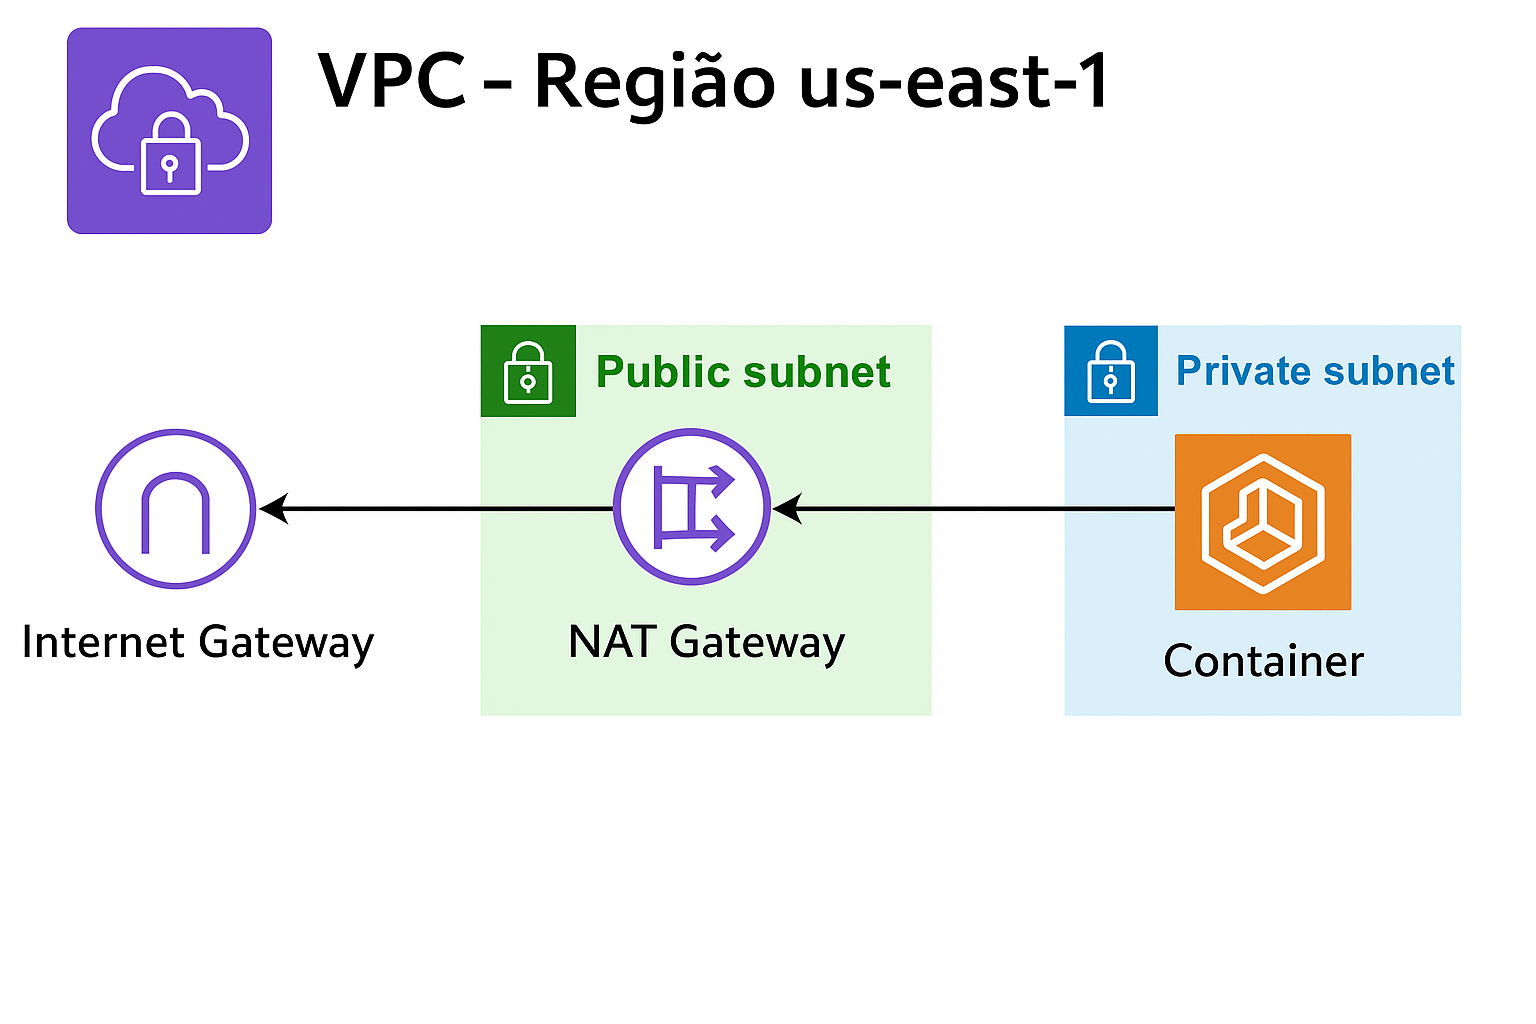
\includegraphics[scale=0.27]{imagens/vpc-simples.png}
}
\legend{Representação da infraestrutura configurada na AWS: o container, alocado em uma subnet privada, acessa a internet por meio de um NAT Gateway posicionado em uma subnet pública.}
\end{figure}


Para garantir a segurança da VPC, é necessária a utilização combinada de Security Groups e Network ACLs (NACLs). Os Security Groups atuam como firewalls com estado, sendo aplicados diretamente às instâncias e permitindo controlar o tráfego de entrada e saída com base em regras dinâmicas. Uma das funcionalidades mais vantajosas dos Security Groups é a possibilidade de fazer referência a outros Security Groups, permitindo que somente instâncias pertencentes a determinados grupos possam se comunicar entre si. Esse recurso facilita a escalabilidade e a gestão centralizada dos acessos na infraestrutura \cite{aws2024securitygroups}.

\subsection{Banco de Dados Gerenciado}\label{sec:metod-rds}
No contexto deste projeto, o banco de dados será acessado a partir do nosso container próprio, por meio de um usuário autenticado com login e senha específicos. Sendo assim, o banco de dados necessita apenas de uma regra de entrada em seu Security Group, permitindo conexões oriundas da aplicação. Todo o controle de autenticação será feito internamente pelo mecanismo de gerenciamento do banco, reforçando a segurança do acesso.

Para garantir alta disponibilidade e evitar pontos únicos de falha na arquitetura, é fundamental distribuir os recursos entre diferentes \textit{Availability Zones} (AZs) dentro de uma mesma região da AWS. Essa abordagem assegura que, caso uma AZ enfrente problemas, as demais possam manter o funcionamento dos serviços, proporcionando resiliência ao sistema.

\subsection{Armazenamento de Objetos}\label{sec:metod-s3}
Embora a resiliência entre regiões (\textit{cross-region}) envolva a replicação de toda a arquitetura em outra região geográfica, o foco deste projeto está na resiliência entre AZs, que oferece um equilíbrio entre disponibilidade e complexidade operacional.

Alguns serviços da AWS são projetados para serem resilientes por padrão. Por exemplo, o \textit{Amazon S3} armazena dados de forma redundante em múltiplas AZs, garantindo alta durabilidade e disponibilidade \cite{netapp2024ha}.

Apesar de o S3 “aparecer” na nossa \textit{região}, ele \textbf{não fica dentro da nossa VPC}. O S3 é um serviço regional da AWS exposto por endpoints públicos, a AWS basicamente “injeta” o serviço na região, mas o bucket não tem IP/ENI na VPC. 

Por isso usamos o VPC Gateway Endpoint, ele cria um alvo lógico nas nossas \textit{route tables} privadas e desvia o tráfego pro S3 por um caminho \textbf{privado}, gerenciado e possuindo alta disponibilidade. 

No entanto, outros serviços requerem configurações específicas para alcançar alta disponibilidade:

\begin{itemize}
  \item \textbf{Amazon RDS}: Para bancos de dados relacionais, é recomendada a implantação \textit{Multi-AZ}, onde uma instância primária é replicada de forma síncrona para uma instância em espera em outra AZ. Em caso de falha, o RDS realiza automaticamente o \textit{failover} para a instância secundária \cite{aws2024rds}.
  
  \item \textbf{Amazon ECS (Fargate)}: Ao utilizar o ECS com Fargate, é possível distribuir as tarefas entre múltiplas AZs, aumentando a resiliência da aplicação.
  
  \item \textbf{NAT Gateway}: Para permitir que instâncias em sub-redes privadas acessem a internet, recomenda-se a criação de um NAT Gateway em cada AZ utilizada, evitando dependência de uma única zona e melhorando a disponibilidade \cite{aws2024nat}.
\end{itemize}

\subsection{Arquitetura Geral em 3 Camadas}\label{sec:metod-fig-geral}
Ao adotar essas práticas, a arquitetura do projeto se torna mais robusta e preparada para lidar com falhas em componentes individuais ou em AZs inteiras, garantindo a continuidade dos serviços e a integridade dos dados.

A Figura~\ref{fig:arquitetura-geral}, a seguir apresenta a arquitetura planejada para o projeto, organizada em três camadas distintas: Camada de Balanceamento, Camada de Aplicação e Camada de Banco de Dados. Cada camada está distribuída entre duas sub-redes (Subnet A e Subnet B), refletindo uma estratégia de alta disponibilidade entre Zonas de Disponibilidade (AZs). Essa abordagem garante resiliência e escalabilidade da solução implementada.

\begin{figure}[H]
\centering
\caption{Arquitetura geral do ambiente na AWS}
\label{fig:arquitetura-geral}
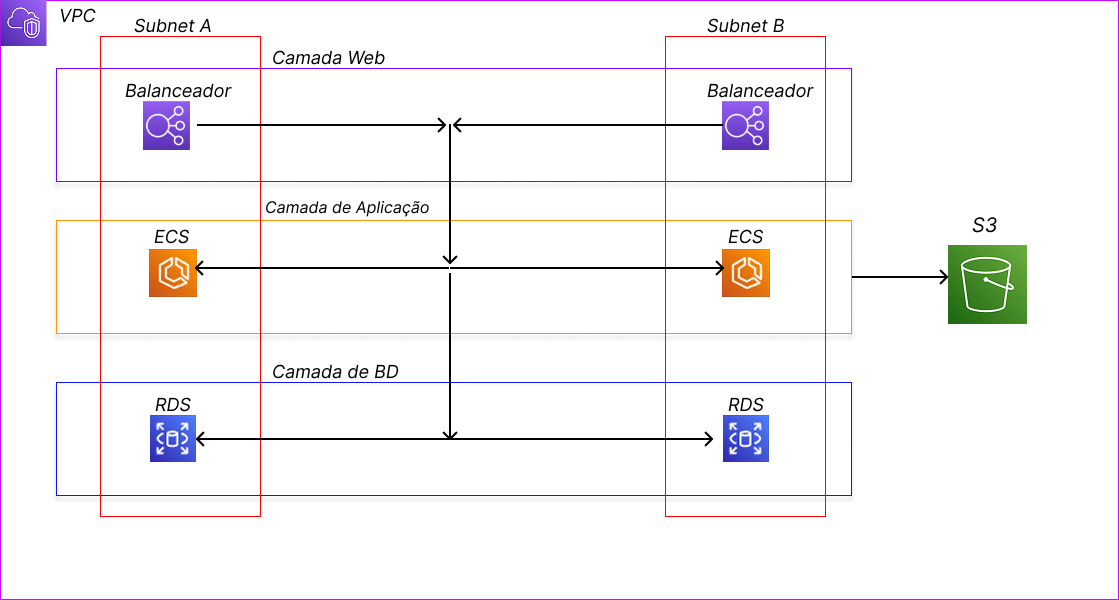
\includegraphics[scale=0.4]{imagens/arquitetura.png}
\legend{Visão em camadas da infraestrutura: balanceamento, aplicação e banco de dados, com distribuição entre duas sub-redes em Zonas de Disponibilidade distintas.}
\end{figure}


Na AWS, a principal ferramenta para implementação de IaC é o \textit{AWS CloudFormation}, que permite descrever toda a infraestrutura em arquivos escritos nos formatos JSON ou YAML. No contexto deste projeto, optou-se pela utilização do formato YAML por sua legibilidade e simplicidade sintática, o que facilita a manutenção e compreensão do código de infraestrutura.\cite{aws2024cloudformation}

Com essa abordagem, todos os recursos utilizados, como VPCs, sub-redes, gateways, grupos de segurança, serviços ECS, RDS e S3, são declarados em um único arquivo, possibilitando o controle de versão, repetibilidade e automação do ambiente de nuvem.




\chapter{Implementação}

\section{Método de implementação}
Conforme citado, foi utilizada a \textbf{Infraestrutura como Código (IaC)} para a construção da nossa arquitetura. O código será detalhado para facilitar o entendimento e servir como documentação para futuras manutenções ou novas implementações. A estrutura geral de cada recurso, incluindo seu nome, tipo e o bloco de propriedades, segue um padrão global no CloudFormation. Por isso, a partir de agora, focaremos apenas nas propriedades que são cruciais e específicas para cada recurso, evitando repetições e tornando a leitura mais objetiva.

\Needspace{2\baselineskip}
\section{VPC}
Com esse trecho, fizemos a criação do nosso recurso Virtual Private Cloud (VPC).
\begin{lstlisting}[language=yaml, float=htbp,]
 VPC:
   Type: AWS::EC2::VPC
   Properties:
     CidrBlock: 10.16.0.0/16
     EnableDnsSupport: true
     EnableDnsHostnames: true
     Tags: [{ Key: Name, Value: TCC-VPC }]
\end{lstlisting}

A seguir, detalhamos cada uma das propriedades do código da VPC:
\begin{description}
    \item[\textbf{VPC:}] É o nome que demos ao recurso. Ele serve como um identificador único, permitindo que outros recursos (como as subnets) o referenciem futuramente no mesmo código.
    \item[\textbf{Type: AWS::EC2::VPC}] Esta é a declaração formal do recurso, especificando que estamos criando uma \textbf{Virtual Private Cloud}.
    \item[\textbf{Properties:}] Este bloco contém todas as configurações e propriedades específicas para o recurso VPC.
    \item[\textbf{CidrBlock:}] Define o bloco de endereços IP da nossa rede e o seu respectivo \textit{range}.
    \item[\textbf{EnableDnsSupport e EnableDnsHostnames:}] Ambas as propriedades, quando definidas como \texttt{true}, ativam o suporte a DNS, permitindo que os recursos dentro da VPC se comuniquem usando nomes de domínio em vez de apenas endereços IP.
    \item[\textbf{Tags:}] São etiquetas ou rótulos que auxiliam na identificação e organização do recurso no console da AWS, de forma visual e intuitiva.
\end{description}
\section{Subnets}
Após a criação da nossa rede principal (\textbf{VPC}), o próximo passo é dividi-la em sub-redes ou \textbf{subnets}. Para o nosso projeto, criamos uma subnet pública (para recursos com acesso à internet) e uma privada (para recursos que devem permanecer isolados).

Para garantir alta disponibilidade e organização, nossa infraestrutura de rede foi planejada com seis subnets distribuídas em duas Zonas de Disponibilidade (AZs). Essa estrutura proporciona redundância e resiliência a falhas.

\begin{enumerate}
    \item Subnet Pública na primeira AZ, para recursos com acesso direto à internet.
    \item Subnet Pública na segunda AZ, servindo ao mesmo propósito na AZ secundária.
    \item Subnet Privada para os containers na primeira AZ, isolando a aplicação da internet.
    \item Subnet Privada para os containers na segunda AZ, garantindo a resiliência do ambiente.
    \item Subnet Privada para o banco de dados na primeira AZ, assegurando o máximo de isolamento e segurança.
    \item Subnet Privada para o banco de dados na segunda AZ, com a mesma finalidade na AZ de backup.
\end{enumerate}

\subsection{Subnet Pública}
Esta subnet foi criada para hospedar recursos que precisam ser acessíveis publicamente, como servidores web ou balanceadores de carga.

\Needspace{2\baselineskip}
\begin{lstlisting}[language=yaml, float=htbp]
 PublicSubnetA:
   Type: AWS::EC2::Subnet
   Properties:
     AvailabilityZone: !Select [0, !GetAZs '']
     VpcId: !Ref VPC
     CidrBlock: 10.16.0.0/20
     Tags: [{ Key: Name, Value: PublicSubnetA }]
\end{lstlisting}


\begin{description}
\item[\textbf{VpcId: !Ref VPC}] Esta propriedade é crucial. Ela utiliza a função intrínseca \texttt{!Ref} para referenciar o recurso \textbf{VPC} que definimos anteriormente. Isso garante que esta subnet seja criada dentro do ambiente de rede que configuramos.
\item[\textbf{AvailabilityZone: !Select [0, !GetAZs ' ']}] O campo \texttt{AvailabilityZone} define em qual Zona de Disponibilidade a Subnet será criada. Usamos a função \texttt{!Select [0, !GetAZs ' ']} para selecionar a primeira Zona de Disponibilidade disponível na região, considerando que a contagem de índices começa em 0.
\item[\textbf{CidrBlock:}] Define o bloco de endereços IP para esta subnet. É importante notar que este bloco de endereços, \texttt{10.16.0.0/20}, é um sub-bloco extraído do \textit{range} maior da nossa VPC, \texttt{10.16.0.0/16}, garantindo que ele não se sobreponha a outras subnets.
\end{description}

\subsection{Vínculo do IGW com a VPC}
Percebemos que a exposição da subnet não é decidida no momento de sua criação, somente quando a associamos a recursos que se conectam com a internet pública, como o IGW, como mostrado a seguir.

\Needspace{2\baselineskip}
\begin{lstlisting}[language=yaml, float=htbp]
 IGW:
   Type: AWS::EC2::InternetGateway
   Properties:
     Tags: [{ Key: Name, Value: TCC-IGW }]
\end{lstlisting}

\Needspace{2\baselineskip}
\begin{lstlisting}[language=yaml, float=htbp]
 AttachIGW:
   Type: AWS::EC2::VPCGatewayAttachment
   Properties:
     VpcId: !Ref VPC
     InternetGatewayId: !Ref IGW
\end{lstlisting}
Com essa sequência de imagens, podemos observar a criação e o vínculo do nosso Internet Gateway com a nossa VPC, processo que se dá por meio das seguintes características:
\begin{description}
\item [\textbf{VpcId: !Ref VPC}] onde referenciamos a VPC que será vinculada.
\item [\textbf{InternetGatewayId: !Ref IGW}] onde referenciamos o Internet Gateway que será utilizado.
\end{description}


\subsection{Criação da Tabela de Rotas e suas Rotas}
Nesse trecho de código é criado a Tabela e sua regra, respectivamente.
\Needspace{2\baselineskip}
\begin{lstlisting}[language=yaml, float=htpb]
 Type: AWS::EC2::RouteTable
   Properties:
     VpcId: !Ref VPC
     Tags: [{ Key: Name, Value: Public-RT }]
\end{lstlisting}

\Needspace{2\baselineskip} % reserva espaço; ajuste o 2 se precisar
\begin{lstlisting}[language=YAML, float=htbp, label={lst:public-default}]
PublicDefaultRoute:
  Type: AWS::EC2::Route
  Properties:
    RouteTableId: !Ref PublicRT
    DestinationCidrBlock: 0.0.0.0/0
    GatewayId: !Ref IGW
\end{lstlisting}

\begin{description}
\item [\textbf{RouteTableId: !Ref PublicRT}] onde apontamos a tabela na qual essa regra será inserida.
\item [\textbf{DestinationCidrBlock: 0.0.0.0/0}] Isso significa que quaisquer pacotes de dados, com qualquer endereço, são incluídos nesta regra. O valor \texttt{0.0.0.0/0} é conhecido como um caminho que engloba todos os pacotes.
\item [\textbf{GatewayId: !Ref IGW}] é onde referenciamos o destino para o qual os pacotes serão enviados.
\end{description}

\subsection{Associação da Tabela de Rotas com a Subnet}
Depois de criar a \textbf{tabela de rotas} e suas \textbf{rotas} (incluindo a \texttt{0.0.0.0/0} para o IGW, no caso de subnet pública), fazemos a \textbf{associação} da tabela à subnet. É essa ligação que, na prática, define o comportamento da subnet: pública (default via IGW), privada com saída (default via NAT) ou isolada (sem default).

\Needspace{2\baselineskip} % reserva espaço; ajuste o 2 se precisar
\begin{lstlisting}[language=YAML, float=htbp]
AssocPublicA:
  Type: AWS::EC2::SubnetRouteTableAssociation
  Properties:
    SubnetId: !Ref PublicSubnetA
    RouteTableId: !Ref PublicRT
\end{lstlisting}

\begin{description}
  \item[\textbf{SubnetId: !Ref PublicSubnetA}] Qual subnet estamos vinculando.
  \item[\textbf{RouteTableId: !Ref PublicRT}] Qual tabela de rotas a subnet vai usar.
\end{description}

\subsection{Visão Geral Pública}
Com as configurações concluídas, a Figura~\ref{fig:rt-publica} resume o ponto-chave: 
\textbf{na tabela de rotas pública, a rota \texttt{0.0.0.0/0} aponta para o IGW}. 
Quando essa tabela é \textbf{associada} à subnet, ela passa a ter saída/entrada pela Internet (respeitando SG/NACL).

\begin{figure}[H]
\centering
\caption{Route table pública com rota \texttt{0.0.0.0/0} para o IGW}
\label{fig:rt-publica}
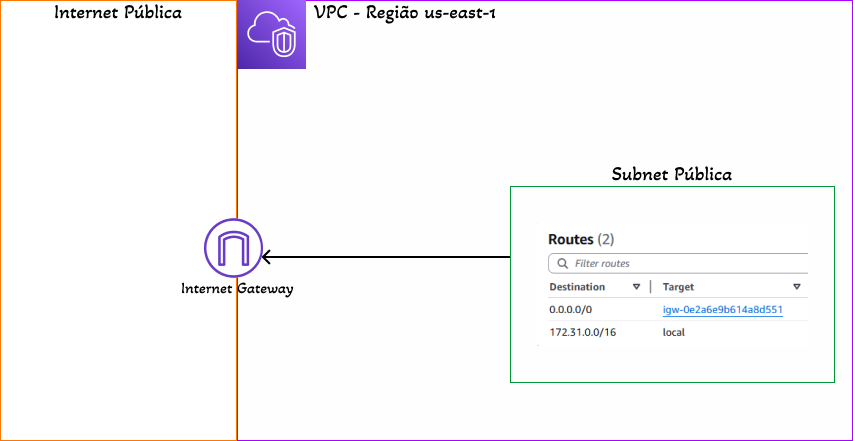
\includegraphics[scale=0.5]{imagens/SubnetPublica.png}
\legend{A rota \texttt{0.0.0.0/0} encaminha o tráfego para o \textit{Internet Gateway} (IGW). 
Ao associar esta tabela à subnet, ela se torna \textbf{pública}.}
\end{figure}


\subsection{Subnet Privada}
Esta subnet hospeda recursos que \textbf{não devem ser expostos diretamente à internet}. Aqui, o tráfego é \textbf{somente de dentro para fora} (saída); conexões \textbf{de fora para dentro} não entram pela internet pública, pois a rota default aponta para um \textit{NAT Gateway}, e não para o \textit{Internet Gateway}.

\Needspace{2\baselineskip}
\begin{lstlisting}[language=YAML,float=htbp,label={lst:subnet-priv-a}]
AppPrivateSubnetA:
  Type: AWS::EC2::Subnet
  Properties:
    AvailabilityZone: !Select [0, !GetAZs '']
    VpcId: !Ref VPC
    CidrBlock: 10.16.32.0/20
    Tags: [{ Key: Name, Value: AppPrivateSubnetA }]
\end{lstlisting}

\begin{description}
  \item[\textbf{AvailabilityZone: !Select [0, !GetAZs '']}] fixa a subnet na \textbf{primeira AZ} da região (índice 0), garantindo distribuição determinística.
  \item[\textbf{VpcId: !Ref VPC}] cria a subnet \textbf{dentro} da VPC definida.
  \item[\textbf{CidrBlock: 10.16.32.0/20}] bloco IP sem sobreposição com as demais sub-redes (recorte do /16 da VPC).
\end{description}

Para saída segura (updates, pull de imagem, etc.), usamos um \textbf{NAT Gateway} com um \textbf{EIP} (IP público fixo). O NAT fica em \textbf{subnet pública} e não aceita conexões iniciadas de fora para dentro, ele apenas \textbf{traduz} o tráfego \emph{originado} das subnets privadas.

\Needspace{2\baselineskip} % reserva espaço; ajuste o 2 se precisar
\begin{lstlisting}[language=YAML, float=htbp]
NatEIPA:
  Type: AWS::EC2::EIP
  Properties:
    Domain: vpc
\end{lstlisting}

\begin{description}
  \item[\textbf{Domain: vpc}] aloca o EIP no escopo da \textbf{VPC}. Esse EIP será o \textbf{IP público fixo} do NAT.
\end{description}

\Needspace{2\baselineskip} % reserva espaço; ajuste o 2 se precisar
\begin{lstlisting}[language=YAML, float=htbp]
NATGWA:
  Type: AWS::EC2::NatGateway
  Properties:
    AllocationId: !GetAtt NatEIPA.AllocationId
    SubnetId: !Ref PublicSubnetA
    Tags: [{ Key: Name, Value: NATGW-A }]
\end{lstlisting}

\begin{description}
  \item[\textbf{AllocationId: !GetAtt NatEIPA.AllocationId}] \textbf{vincula} o EIP ao NAT (garante IP público estável para o tráfego de saída).
  \item[\textbf{SubnetId: !Ref PublicSubnetA}] o NAT \textbf{deve ficar em subnet pública} (pois precisa falar com a internet via IGW).
\end{description}

Criamos então a \textbf{route table privada} da AZ A e apontamos a \textbf{rota default (0.0.0.0/0)} para o \textbf{NAT Gateway}, é isso que dá à subnet privada \textbf{saída para a internet} sem exposição de entrada.

\Needspace{2\baselineskip} % reserva espaço; ajuste o 2 se precisar
\begin{lstlisting}[language=YAML, float=htbp]
PrivateRTA:
  Type: AWS::EC2::RouteTable
  Properties:
    VpcId: !Ref VPC
    Tags: [{ Key: Name, Value: Private-RT-A }]
\end{lstlisting}

\Needspace{2\baselineskip} % reserva espaço; ajuste o 2 se precisar
\begin{lstlisting}[language=YAML, float=htbp]
PrivateDefaultRouteA:
  Type: AWS::EC2::Route
  Properties:
    RouteTableId: !Ref PrivateRTA
    DestinationCidrBlock: 0.0.0.0/0
    NatGatewayId: !Ref NATGWA
\end{lstlisting}

\begin{description}
  \item[\textbf{RouteTableId: !Ref PrivateRTA}] indica \textbf{em qual tabela} a rota será criada (a “privada A”).
  \item[\textbf{DestinationCidrBlock: 0.0.0.0/0}] \textbf{tudo que não for rede interna} (default) segue esta rota.
  \item[\textbf{NatGatewayId: !Ref NATGWA}] define o \textbf{alvo} da default como o NAT (saída \emph{egress} apenas).
\end{description}

Por fim, associamos a \textbf{subnet privada} à \textbf{sua route table privada} (mesma lógica do caso público; só mudamos IGW→NAT). Sem essa associação, a subnet herdaria a \textit{main route table}.

\Needspace{2\baselineskip} % reserva espaço; ajuste o 2 se precisar
\begin{lstlisting}[language=YAML, float=htbp]
AssocAppAtoRTA:
    Type: AWS::EC2::SubnetRouteTableAssociation
    Properties:
      SubnetId: !Ref AppPrivateSubnetA
      RouteTableId: !Ref PrivateRTA
\end{lstlisting}

\subsection{Visão Geral Privada}
A seguir, a Figura~\ref{fig:rt-privada} apresenta a parte \textbf{privada} da arquitetura:
a subnet de aplicação com rota \texttt{0.0.0.0/0} apontando para o \textbf{NAT Gateway}.

\begin{figure}[H]
\centering
\caption{Route table \textbf{privada} com rota \texttt{0.0.0.0/0} para o NAT Gateway}
\label{fig:rt-privada}
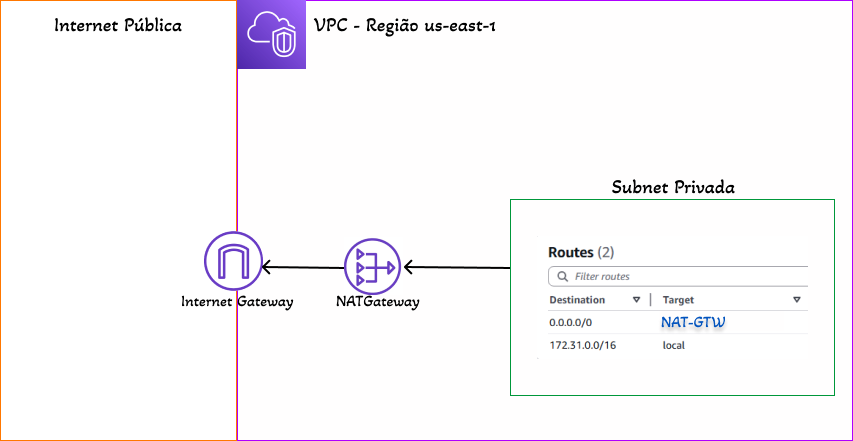
\includegraphics[scale=0.5]{imagens/SubnetPrivada.png}
\legend{A default \texttt{0.0.0.0/0} vai para o \textbf{NAT Gateway} (na subnet pública da \textbf{mesma AZ}),
garantindo \textbf{saída} à Internet via IGW sem expor \textbf{entrada} direta.}
\end{figure}


\section{Grupos de Segurança}
Precisamos criar \textit{Security Groups} (SGs), que são nossos firewalls com estado dentro da VPC. Eles protegem o tráfego e também servem como referência entre recursos: eu defino que “só quem estiver no SG X pode falar com o recurso Y”. Assim, controlo entrada e saída de forma simples e direta, sem abrir portas desnecessárias.

Vamos usar SGs para os nossos principais componentes:

\begin{description}
  \item[\textbf{Balanceador de Carga}] Recebe tráfego público (HTTP/HTTPS) e só encaminha para os containers que estiverem no SG permitido.
  \item[\textbf{Instância do Banco de Dados (RDS)}] Não é pública. Aceita conexões apenas do SG dos containers (porta do banco) e, se necessário, do bastion/jump.
  \item[\textbf{ECS Fargate (Containers)}] Fala com o RDS e com o S3 (via endpoint). Só recebe tráfego do SG do balanceador. Saída liberada apenas para o que precisa.
\end{description}

\Needspace{2\baselineskip} % reserva espaço; ajuste o 2 se precisar
\begin{lstlisting}[language=YAML, float=htbp]
SGALB:
    Type: AWS::EC2::SecurityGroup
    Properties:
      GroupDescription: ALB HTTP
      VpcId: !Ref VPC
      SecurityGroupIngress:
        - { IpProtocol: tcp, FromPort: 80, ToPort: 80, CidrIp: 0.0.0.0/0 }
      SecurityGroupEgress:
        - { IpProtocol: -1, FromPort: 0, ToPort: 0, CidrIp: 0.0.0.0/0 }
\end{lstlisting}

\textbf{GroupDescription: ALB HTTP} Cria uma descrição para o nosso Grupo de Segurança.

\textbf{SecurityGroupIngress: - { IpProtocol: tcp, FromPort: 80, ToPort: 80, CidrIp: 0.0.0.0/0 }} Libera \textbf{todo} tráfego de saída (qualquer protocolo/porta/destino)
        
\textbf{SecurityGroupEgress: - { IpProtocol: -1, FromPort: 0, ToPort: 0, CidrIp: 0.0.0.0/0 }} Libera \textbf{todo} tráfego de saída (qualquer protocolo/porta/destino)

\section{S3 Endpoint Gateway}
Criaremos a nosso S3 Endpoint Gateway, precisamos garantir que ele esteja em duas zonas de disponibilidade, para garantir alta disponibilidade.

\begin{figure}[H]
\centering
\caption{Acesso do container ao S3 via \textbf{Gateway Endpoint} (privado, sem IGW/NAT)}
\label{fig:rt-privada}
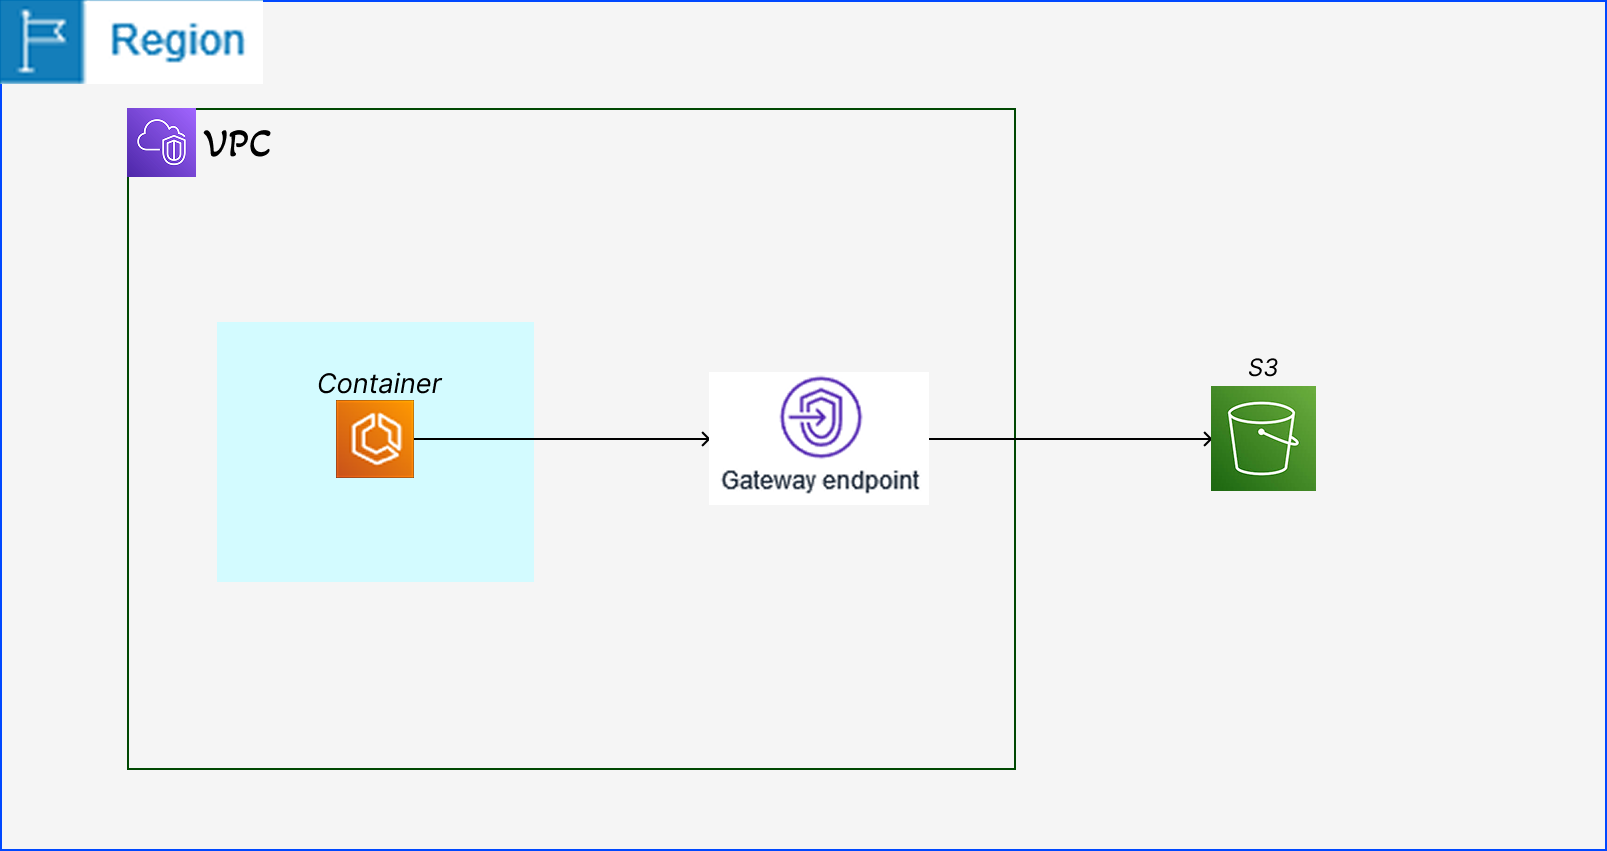
\includegraphics[scale=0.25]{imagens/VPC-Endpoint.png}
\legend{O tráfego ao S3 sai da VPC pelas \textit{route tables} privadas apontando para o \textbf{Gateway Endpoint} do S3. Não há exposição à Internet, nem uso de NAT; o caminho é gerenciado e altamente disponível por padrão.}
\end{figure}

\Needspace{10\baselineskip} % reserva espaço; ajuste o 2 se precisar
\begin{lstlisting}[language=YAML]
S3GatewayEndpoint:
    Type: AWS::EC2::VPCEndpoint
    Properties:
      VpcId: !Ref VPC
      ServiceName: !Sub com.amazonaws.${AWS::Region}.s3
      VpcEndpointType: Gateway
      RouteTableIds: [ !Ref PrivateRTA, !Ref PrivateRTB ]
      PolicyDocument:
        Version: '2012-10-17'
        Statement:
          - Effect: Allow
            Principal: "*"
            Action: "s3:*"
            Resource: "*"
\end{lstlisting}


\textbf{ServiceName: !Sub com.amazonaws.\${AWS::Region}.s3} Nome do serviço do S3 na região (prefix list regional).

\textbf{VpcEndpointType: Gateway} Escolhemos \textit{Gateway} (e não \textit{Interface}) porque é o tipo próprio do S3: usa rotas nas \textit{route tables}, não precisa SG, não exige ENI por AZ e não tem cobrança por hora do endpoint — fica mais simples e barato pro nosso caso.

\textbf{RouteTableIds: [ PrivateRTA, PrivateRTB ]} Associa o endpoint às RTs privadas; assim, o tráfego pro S3 sai por caminho privado (sem IGW/NAT).

\textbf{PolicyDocument} É a política anexada ao recurso, nesse caso o endpoint. Define quem pode usar este caminho privado e para quais ações no S3.

\textbf{Version: \texttt{2012-10-17}} Versão do schema da política da AWS. Mantemos este valor porque é o padrão atual da linguagem de políticas.

\textbf{Statement} Bloco que contém as regras.

\textbf{Effect: \texttt{Allow}} Diz que a regra \textit{permite}. Se fosse \texttt{Deny}, bloquearia, independentemente de outras permissões.

\textbf{Principal: \texttt{"*"}} Quem está autorizado a usar o recurso. Com asterisco, qualquer principal autenticado que alcance o recurso na VPC pode tentar usar.

\textbf{Action: \texttt{"s3:*"}} Conjunto de operações no S3 liberadas por este caminho. Com asterisco, libera todas as ações.

\textbf{Resource: \texttt{"*"}} Alvos das ações. Com asterisco, vale para qualquer bucket e qualquer objeto, tendo a opção de restriginr os recursos, separando por pastas.

\section{Balanceador de Carga}
Aqui é a “porta de entrada” do usuário. O ALB recebe as requisições e distribui entre os nossos containers. Quando utilizamos o cloudformation, é separado em três partes.

\subsection{Load Balancer}
Nesta etapa criamos o recurso principal do balanceador e definimos as características base.\\

\Needspace{10\baselineskip}
\begin{lstlisting}[language=YAML]
ALB:
  Type: AWS::ElasticLoadBalancingV2::LoadBalancer
  Properties:
    Scheme: internet-facing
    Type: application
    Subnets: [ !Ref PublicSubnetA, !Ref PublicSubnetB ]
    SecurityGroups: [ !Ref SGALB ]
\end{lstlisting}

\textbf{Scheme: internet-facing} É o nosso ponto público. Como o usuário acessa de fora, o ALB precisa ser \textit{internet-facing}. Se fosse \textit{internal}, ficaria restrito à VPC.

\textbf{Type: application} Escolhemos \textit{application} (ALB), que trabalha em camada 7 (HTTP/HTTPS) e entende coisas como caminho, host e headers. O outro tipo é \textit{network} (NLB), camada 4, focado em TCP/UDP e baixa latência.

\textbf{Subnets: [ !Ref PublicSubnetA, !Ref PublicSubnetB ]} Colocamos o ALB em subnets \textbf{públicas} de duas AZs para alta disponibilidade e IPs públicos gerenciados.

\textbf{SecurityGroups: [ !Ref SGALB ]} SG anexado ao ALB.

\subsection{Listener}
É o ponto onde o balanceador de carga escuta as requisições. Aqui se define de onde virão e como serão atendidas as requisições dos clientes.\\

\Needspace{10\baselineskip}
\begin{lstlisting}[language=YAML]
Listener80:
  Type: AWS::ElasticLoadBalancingV2::Listener
  Properties:
    LoadBalancerArn: !Ref ALB
    Port: 80
    Protocol: HTTP
    DefaultActions:
      - Type: forward
        TargetGroupArn: !Ref TargetGroup
\end{lstlisting}

\textbf{LoadBalancerArn: !Ref ALB} Referencia em qual balanceador de carga o listener será criado.

\textbf{Port: 80} Informa a porta que será escutada.

\textbf{Protocol: HTTP} Define o protocolo que será escutado.

\textbf{DefaultActions:} Define o que fazer com as requisições que chegarem.

\textbf{- Type: forward} Diz que as requisições devem ser encaminhadas.

\textbf{TargetGroupArn: !Ref TargetGroup} Indica para onde o tráfego será encaminhado.

\subsection{Target Group}
É a forma de agrupar os containers. Ao criar os containers, eles são associados a um Target Group, e o balanceador usa isso para distribuir as requisições.\\

\Needspace{10\baselineskip}
\begin{lstlisting}[language=YAML]
TargetGroup:
  Type: AWS::ElasticLoadBalancingV2::TargetGroup
  Properties:
    VpcId: !Ref VPC
    Protocol: HTTP
    Port: 8080
    TargetType: ip
    HealthCheckPath: /healthcheck
    Matcher: { HttpCode: 200-399 }
\end{lstlisting}

\textbf{VpcId: !Ref VPC} Define em qual VPC o Target Group está.

\textbf{Protocol: HTTP} Informa o protocolo usado entre o ALB e os destinos.

\textbf{Port: 8080} Porta em que os containers responderão.

\textbf{TargetType: ip} Tipo de destino definido como IP.

\textbf{HealthCheckPath: /healthcheck} Caminho usado para o health check, um “ping” básico para verificar se está respondendo.

\textbf{Matcher: \{ HttpCode: 200-399 \}} Intervalo de códigos considerados sucesso no health check.

\begin{figure}[H]
\centering
\caption{ALB encaminhando tráfego para o \textbf{Target Group} (destinos IP na porta 8080)}
\label{fig:load-balancer}
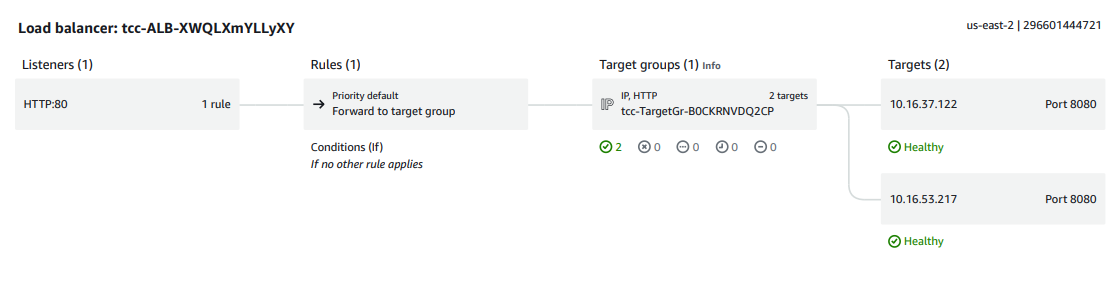
\includegraphics[scale=0.4]{imagens/targets.png}
\legend{Os destinos aparecem como \textit{healthy} após passarem no \textit{health check} definido no Target Group. O balanceamento ocorre a partir do listener HTTP:80.}
\end{figure}

\section{Armazenamento de Objetos}
Será provisionado um bucket S3 para armazenamento de objetos. 
A seção é dividida em duas partes: a criação do recurso e a definição das permissões.\\

\Needspace{10\baselineskip}
\begin{lstlisting}[language=YAML]
MediaBucket:
    Type: AWS::S3::Bucket
    Properties:
      BucketName: !If
        - HasBucketName
        - !Ref MediaBucketName
        - !Sub tcc-flask-media-${AWS::AccountId}-${AWS::Region}
\end{lstlisting}

\textbf{BucketName: !If}

\textbf{ - HasBucketName,} 

\textbf{ - \!Ref MediaBucketName,}

\textbf{ - \!Sub tcc-flask-media-\${AWS::AccountId}-\${AWS::Region}}

Define o nome do bucket. Se um nome for informado no parâmetro \texttt{MediaBucketName}, usa esse valor. Caso contrário, usa o padrão com conta e região.

\Needspace{10\baselineskip}
\begin{lstlisting}[language=YAML]
MediaBucketPolicy:
    Type: AWS::S3::BucketPolicy
    Properties:
      Bucket: !Ref MediaBucket
      PolicyDocument:
        Version: '2012-10-17'
        Statement:
          - Sid: DenyInsecureTransport
            Effect: Deny
            Principal: "*"
            Action: "s3:*"
            Resource:
              - !Sub arn:aws:s3:::${MediaBucket}
              - !Sub arn:aws:s3:::${MediaBucket}/*
            Condition:
              Bool: { aws:SecureTransport: "false" }
\end{lstlisting}


\textbf{Bucket: \texttt{!Ref MediaBucket}} Indica em qual bucket a política será anexada.

\textbf{PolicyDocument} Documento da política em si. É aqui que se define o que é permitido ou negado.

\textbf{Version: \texttt{'2012-10-17'}} Versão do formato da política da AWS. Valor padrão, não altera o comportamento das regras.

\textbf{Statement} Conjunto de regras. 

\textbf{Sid} é só um rótulo legível para identificar a regra.

\textbf{Effect} Define o resultado da regra: \texttt{Allow} para permitir, \texttt{Deny} para negar. Neste caso está como \texttt{Deny}.

\textbf{Principal} Quem está fazendo a chamada. O caractere \texttt{"*"} significa “qualquer principal”.

\textbf{Action} Quais operações a regra cobre. \texttt{"s3:*"} significa “todas as ações do S3”.

- !Sub arn:aws:s3:::\${MediaBucket}

- !Sub arn:aws:s3:::\${MediaBucket}/*

\textbf{Resource} Em quais recursos a regra se aplica. Aqui cobre o bucket raiz.


\section{ECS Fargate - Containers}
A criação das instâncias de containers é organizada em cinco partes: (i) o cluster, que concentra a execução; (ii) o destino dos logs, para facilitar análise em caso de falhas; (iii) as credenciais, separadas em duas funções para manter clareza e granularidade; (iv) a definição da task, onde se especificam propriedades do container e variáveis de ambiente; (v) o service, que define sub-redes de lançamento, quantidade de containers e os vínculos. 

\subsection{Cluster}
No contexto do ECS, o \textit{cluster} é o agrupador lógico onde ficam registrados os serviços e as tasks.

\Needspace{10\baselineskip}
\begin{lstlisting}[language=YAML]
ECSCluster:
  Type: AWS::ECS::Cluster
  Properties:
    ClusterName: flask-ecs-cluster
\end{lstlisting}

\textbf{ClusterName: flask-ecs-cluster} Define o nome lógico do cluster onde os serviços e tasks serão executados.

\subsection{Logs}
Logs registram os eventos de execução do container.
 

\Needspace{10\baselineskip}
\begin{lstlisting}[language=YAML]
LogGroup:
  Type: AWS::Logs::LogGroup
  Properties:
    LogGroupName: /ecs/flask
    RetentionInDays: 7
\end{lstlisting}

\textbf{LogGroupName: /ecs/flask} Nome do grupo de logs para registrar a saída dos containers.

\textbf{RetentionInDays: 7} Define retenção de logs por 7 dias.

\subsection{Credencial de Execução}
Função usada pelo \textit{runtime} do ECS/Fargate durante a execução da task.

\Needspace{10\baselineskip}
\begin{lstlisting}[language=YAML]
ECSExecutionRole:
  Type: AWS::IAM::Role
  Properties:
    AssumeRolePolicyDocument:
      Version: '2012-10-17'
      Statement:
        - Effect: Allow
          Principal: { Service: ecs-tasks.amazonaws.com }
          Action: sts:AssumeRole
    ManagedPolicyArns:
      - arn:aws:iam::aws:policy/service-role/AmazonECSTaskExecutionRolePolicy
\end{lstlisting}

\textbf{AssumeRolePolicyDocument} Autoriza o serviço \texttt{ecs-tasks.amazonaws.com} a assumir a função.

\textbf{Action: sts:AssumeRole} É a linha que afirma que o nosso container pode assumir a nossa Role.

\textbf{ManagedPolicyArns} Anexa a política gerenciada usada na execução das tasks.


\subsection{Credencial da Tarefa}
Função assumida pelo processo dentro do container.

\Needspace{2\baselineskip}
\begin{lstlisting}[language=YAML]
ECSTaskRole:
  Type: AWS::IAM::Role
  Properties:
    AssumeRolePolicyDocument:
      Version: '2012-10-17'
      Statement:
        - Effect: Allow
          Principal: { Service: ecs-tasks.amazonaws.com }
          Action: sts:AssumeRole
    Policies:
      - PolicyName: S3UploadsAccess
        PolicyDocument:
          Version: '2012-10-17'
          Statement:
            - Sid: ListOnBucketPrefix
              Effect: Allow
              Action: ["s3:ListBucket"]
              Resource: !Sub arn:aws:s3:::${MediaBucket}
              Condition:
                StringLike:
                  s3:prefix: [ !Sub "${MediaPrefix}/*" ]
            - Sid: RWOnPrefix
              Effect: Allow
              Action: ["s3:GetObject","s3:PutObject","s3:DeleteObject"]
              Resource: !Sub arn:aws:s3:::${MediaBucket}/${MediaPrefix}/*
\end{lstlisting}

\textbf{AssumeRolePolicyDocument} Permite que as tasks assumam a função.

\textbf{Policies \(\rightarrow\) S3UploadsAccess} Concede acesso mínimo necessário ao bucket de mídias. Priorizando segurança.

\textbf{ListOnBucketPrefix} Autoriza listar o bucket apenas no prefixo informado.

\textbf{RWOnPrefix} Autoriza leitura e escrita de objetos somente no prefixo definido.



\subsection{Task}
Descreve como o container será executado: compatibilidade, recursos, rede, permissões.

\begin{lstlisting}[language=YAML]
TaskDefinition:
    Type: AWS::ECS::TaskDefinition
    DependsOn: [ MySQLInstance ]
    Properties:
      RequiresCompatibilities: [ FARGATE ]
      Cpu: 512
      Memory: 1024
      NetworkMode: awsvpc
      ExecutionRoleArn: !GetAtt ECSExecutionRole.Arn
      TaskRoleArn: !GetAtt ECSTaskRole.Arn
      ContainerDefinitions:
        - Name: flask
          Image: !Ref ECRImage
          PortMappings:
            - ContainerPort: 8080
          Environment:
            ...
          LogConfiguration:
            LogDriver: awslogs
            Options:
              awslogs-group: /ecs/flask
              awslogs-region: !Ref AWS::Region
              awslogs-stream-prefix: app
          HealthCheck:
            Command: ["CMD-SHELL", "curl -fsS http://localhost:8080/healthcheck || exit 1"]
            Interval: 30
            Timeout: 5
            Retries: 3
            StartPeriod: 10
\end{lstlisting}

\textbf{DependsOn: [ MySQLInstance]} Garante a ordem de criação: a task só é criada após a instância do banco. 
\textit{Nota:} isso não garante que o banco já esteja “pronto” para conexões; apenas a criação ocorre depois.

\textbf{RequiresCompatibilities: [ FARGATE ]} Define que a execução é no Fargate (sem gerenciamento de servidor).

\textbf{Cpu: 512} Quantidade de CPU reservada para a task.

\textbf{Memory: 1024} Quantidade de memória reservada para a task (em MiB).

\textbf{NetworkMode: awsvpc} Modo de rede compatível com Fargate. Cada task tem endereço IP próprio na VPC e pode usar Security Group dedicado.

\textbf{ExecutionRoleArn: !GetAtt ECSExecutionRole.Arn} Função usada pelo runtime do ECS (pull da imagem, logs, etc.).

\textbf{TaskRoleArn: !GetAtt ECSTaskRole.Arn} Função assumida pelo processo dentro do container (permissões da aplicação; no caso, acesso ao S3).

\textbf{ContainerDefinitions} Bloco com as características do container que vai rodar.

\quad\textbf{Name: flask} Nome lógico do container.

\quad\textbf{Image: !Ref ECRImage} Imagem utilizada no deploy.

\quad\textbf{PortMappings \(\rightarrow\) ContainerPort: 8080} Porta na qual o container escuta.

\quad\textbf{Environment} Bloco de variáveis de ambiente do container.

\quad\textbf{LogConfiguration \(\rightarrow\) LogDriver: awslogs} Envio de logs para o CloudWatch Logs (\texttt{group}, \texttt{region}, \texttt{stream-prefix}).

\quad\textbf{HealthCheck} Comando para verificação de saúde do container (intervalo, timeout, tentativas e período inicial)..

\subsection{Service}
Definimos a quantidade de instâncias que vamos lançar, as subnets e outros.

\begin{lstlisting}[language=YAML]
Service:
    Type: AWS::ECS::Service
    DependsOn: [ ALB, Listener80, TargetGroup ]
    Properties:
      Cluster: !Ref ECSCluster
      LaunchType: FARGATE
      DesiredCount: 2
      EnableExecuteCommand: true
      TaskDefinition: !Ref TaskDefinition
      NetworkConfiguration:
        AwsvpcConfiguration:
          AssignPublicIp: DISABLED
          Subnets: [ !Ref AppPrivateSubnetA, !Ref AppPrivateSubnetB ]
          SecurityGroups: [ !Ref APPSG ]
      LoadBalancers:
        - ContainerName: flask
          ContainerPort: 8080
          TargetGroupArn: !Ref TargetGroup
\end{lstlisting}

\textbf{DependsOn: [ ALB, Listener80, TargetGroup ]} Garante a criação do ALB, listener e target group antes do service.

\textbf{Cluster: !Ref ECSCluster} Agrupamento onde o service será executado.

\textbf{LaunchType: FARGATE} Tipo de execução do container.

\textbf{DesiredCount: 2} Quantidade de instâncias (tasks) em execução.

\textbf{EnableExecuteCommand: true} Habilita comandos interativos na task (exec).

\textbf{TaskDefinition: !Ref TaskDefinition} Qual definição de task o service vai usar.

\textbf{NetworkConfiguration \(\rightarrow\) AwsvpcConfiguration}
\quad \textbf{AssignPublicIp: DISABLED} Sem IP público para as tasks.

\quad \textbf{Subnets: [ AppPrivateSubnetA, AppPrivateSubnetB ]} Sub-redes privadas onde as tasks serão lançadas.

\quad \textbf{SecurityGroups: [ APPSG ]} Grupo de segurança aplicado nas tasks.

\textbf{LoadBalancers}
\quad \textbf{ContainerName: flask} Container dentro da task que receberá o tráfego.

\quad \textbf{ContainerPort: 8080} Porta do container exposta ao ALB.

\quad \textbf{TargetGroupArn: !Ref TargetGroup} Para onde o ALB encaminha as requisições.


\section{Banco de Dados}
A criação do banco é dividida em duas etapas: primeiro o \textit{Subnet Group}, que define onde a instância pode ser alocada; depois a própria instância, com suas propriedades.

\subsection{Subnet Group — Banco de Dados}

\Needspace{3\baselineskip}
\begin{lstlisting}[language=YAML]
DBSubnetGroup:
  Type: AWS::RDS::DBSubnetGroup
  Properties:
    DBSubnetGroupDescription: Subnets para RDS MySQL
    SubnetIds: [ !Ref DBPrivateSubnetA, !Ref DBPrivateSubnetB ]
\end{lstlisting}

\textbf{DBSubnetGroupDescription: Subnets para RDS MySQL} Descrição do grupo de sub-redes.\\
\textbf{SubnetIds: [ !Ref DBPrivateSubnetA, !Ref DBPrivateSubnetB ]} Sub-redes onde a instância de banco pode ser criada (duas AZs).

\subsection{Instância - Banco de Dados}
Nesta etapa são definidas as propriedades da instância: versão do SGBD, classe de instância, tamanho e tipo de armazenamento, além dos parâmetros básicos de operação. O objetivo é especificar o que será executado e como será alocado o recurso para atender à aplicação.\\

\Needspace{10\baselineskip}
\begin{lstlisting}[language=YAML]
MySQLInstance:
    Type: AWS::RDS::DBInstance
    Properties:
      Engine: mysql
      EngineVersion: "8.0.42"
      DBInstanceClass: db.t4g.micro
      AllocatedStorage: 20
      StorageType: gp3
      MultiAZ: true
      MasterUsername: !Ref DBUser
      MasterUserPassword: !Ref DBPassword
      DBName: !Ref DBName
      VPCSecurityGroups: [ !Ref DBSG ]
      DBSubnetGroupName: !Ref DBSubnetGroup
\end{lstlisting}

\textbf{Engine: mysql} Motor do banco definido como MySQL.

\textbf{EngineVersion: "8.0.42"} Versão utilizada do MySQL.

\textbf{DBInstanceClass: db.t4g.micro} Classe/tamanho da instância (perfil de demonstração).

\textbf{AllocatedStorage: 20} Armazenamento alocado em GiB.

\textbf{StorageType: gp3} Tipo de volume usado pelo RDS.

\textbf{MultiAZ: true} Habilita implantação em múltiplas zonas de disponibilidade, com failover automático.

\textbf{MasterUsername: !Ref DBUser} Usuário principal do banco.

\textbf{MasterUserPassword: !Ref DBPassword} Senha do usuário principal.

\textbf{DBName: !Ref DBName} Nome do database inicial.

\textbf{VPCSecurityGroups: [ !Ref DBSG ]} Grupo(s) de segurança associados à instância.

\textbf{DBSubnetGroupName: !Ref DBSubnetGroup} Sub-redes onde a instância pode ser criada.

\textbf{CopyTagsToSnapshot: true} Replica as tags da instância para os snapshots.


\section{Parâmetros}
Declara os valores que podem ser informados na criação (ou atualização) da pilha, permitindo personalizar o template conforme a necessidade. São valores fornecidos em tempo de implantação e depois referenciados no template pelos recursos que precisam deles.
 
\Needspace{10\baselineskip}
\begin{lstlisting}[language=YAML]
Parameters:
  ECRImage:
    Type: String
    Default: 296601444721.dkr.ecr.us-east-2.amazonaws.com/tcc/flask:latest

  DBName:
    Type: String
    Default: appdb
    Description: Nome do database no RDS MySQL

  DBUser:
    Type: String
    Default: appuser
    Description: Usuário do DB

  DBPassword:
    Type: String
    NoEcho: true
    Description: Senha do DB (8-41 chars)

  MediaBucketName:
    Type: String
    Default: ""
    Description: Nome do bucket S3 para mídias; Em branco, cria um aleatório 

  MediaPrefix:
    Type: String
    Default: "uploads"
    Description: Prefixo (caminho) para objetos no S3

Conditions:
  HasBucketName: !Not [ !Equals [ !Ref MediaBucketName, "" ] ]
\end{lstlisting}


\textbf{ECRImage} Nome do parâmetro usado para referência no template (via \texttt{!Ref}); aqui guarda a URI da imagem no ECR.

\textbf{Type: String} Tipo do parâmetro no CloudFormation. Existindo. Há String e Number.

\textbf{Default: 296601444721.dkr.ecr.us-east-2.amazonaws.com/tcc/flask:latest} Valor padrão. Se o usuário não informar nada, será usada essa imagem Docker.

\chapter{Conclusão}
\label{sec:conclusao}

\section{Necessidades do projeto}
Para reproduzir a arquitetura proposta, recomenda-se conhecimento básico em redes e contêineres, já que é necessário dispor de uma imagem pronta para implantação. Com esses fundamentos, a solução pode ser ajustada conforme a aplicação: por exemplo, em cenários com front-end e back-end separados, é possível usar \textbf{um único ALB} com regra de roteamento (por caminho/host/porta) para direcionar o tráfego a \textit{target groups} distintos, ou optar por \textbf{dois ALBs}, um público para o front-end e outro interno para o back-end.


\section{Implementação da Arquitetura}
Toda a arquitetura foi implementada via IaC (Infraestrutura como Código), utilizando um template CloudFormation e uma imagem Docker personalizada. A imagem própria facilita a demonstração, pois expõe a estrutura do aplicativo e permite adaptar o conteúdo ao projeto de forma direta.

A opção pelo CloudFormation tem como principais motivos:
\begin{itemize}
  \item Padronização do conteúdo;
  \item Fácil replicação;
  \item Redução de erros humanos;
  \item Atualização e manutenção simplificadas dos componentes.
\end{itemize}

\section{Estimativa de custos (modelo de cálculo)}
Abaixo segue um \textit{modelo} de tabela para estimar o custo mensal da solução \textit{na AWS} e uma visão equivalente \textit{on-premises} mensalizada. Os valores são apenas estipulações, variando de necessidade para necessidade.

\begin{table}[H]
\centering
\caption{Custo mensal estimado — AWS (exemplo ilustrativo, \textbf{R\$})}
\label{tab:custo-aws-brl}
\begin{tabular}{|p{5cm}|p{7cm}|p{4cm}|}
\hline
\textbf{Componente} & \textbf{Hipótese de consumo} & \textbf{Estimativa (R\$/mês)} \\
\hline
ALB (Application Load Balancer) & 730 h + \(\sim\)1 LCU/h (tráfego baixo) & R\$~129 \\
\hline
ECS Fargate (2 tasks) & 2x (0{,}5 vCPU, 1 GB) por 730 h & R\$~192 \\
\hline
RDS MySQL (db.t4g.micro, Multi-AZ) & 730 h (ativo+standby) & R\$~125 \\
\hline
RDS Storage (gp3) & 20 GB & R\$~12 \\
\hline
S3 (mídias) & 20 GB + requests leves & R\$~2{,}45 \\
\hline
CloudWatch Logs & 1 GB ingerido/mês & R\$~2{,}67 \\
\hline
NAT Gateway & 730 h + 10 GB processados & R\$~177{,}5 \\
\hline
Data Transfer Out (Internet) & 10 GB/mês & R\$~4{,}80 \\
\hline
\multicolumn{2}{|r|}{\textbf{Total (com NAT)}} & \textbf{R\$~645} \\
\hline
\end{tabular}
\end{table}



\begin{table}[H]
\centering
\caption{Custo mensal equivalente — On-Premises no Brasil (exemplo, \textbf{R\$})}
\label{tab:custo-onprem-brl}
\begin{tabular}{|p{5cm}|p{7cm}|p{4cm}|}
\hline
\textbf{Item} & \textbf{Hipótese (referências BR)} & \textbf{Mensal (R\$)} \\
\hline
Servidor (compute) & Dell PowerEdge T150 de entrada \(\sim\)R\$ 7{,}1 mil (amort. 36 meses) & \textbf{R\$ 197} \\
\hline
Armazenamento local & Discos/SSD inclusos básicos (já no T150) — extra conforme projeto & \textbf{—} \\
\hline
Energia elétrica (TI) & Ex.: 150 W médios \(\approx\) 108 kWh/mês; tarifa + bandeira (estim.) & \textbf{R\$ 117} \\
\hline
Resfriamento/overhead & Regra simples 1:1 com energia de TI (estim.) & \textbf{R\$ 117} \\
\hline
Link empresarial & Internet/Link dedicado: a partir de \textasciitilde R\$ 500–700/mês (30–50 Mb) & \textbf{R\$ 600} \\
\hline
Firewall/UTM & Fortigate 60F + licença UTP 12 meses \(\sim\)R\$ 5{,}538 (= R\$ 462/mês) & \textbf{R\$ 462} \\
\hline
Administração/Operação & 4–6 h/mês (estimativa conservadora) & \textbf{R\$ 1{,}000} \\
\hline
\multicolumn{2}{|r|}{\textbf{Total (on-premises)}} & \textbf{R\$ 2{,}493} \\
\hline
\end{tabular}
\end{table}



\section{Considerações finais}
A solução apresentada tem complexidade média, porém segue padrões claros que servem de apoio ao leitor. Com a leitura detalhada deste documento, é possível implantar uma arquitetura robusta, completa e segura, sem exigir estudo extensivo.

Em suma, a arquitetura proposta atende a requisitos típicos de ambiente empresarial e pode ser implementada com conhecimentos básicos, conforme descrito no início do capítulo. Assim, o objetivo do trabalho foi alcançado.




%%%%%%%%%%%%%%%%%%%%%%%%%%%%%%%%%%%%%%%%%%%%%%%%%%%%%%%%%%%%%%%%%%%%%%%%%%%%%%%%
%%% Elementos pós-textuais
\postextual

% Referências bibliográficas: OBRIGATÓRIO.
% Indique, abaixo, onde está o banco de dados (geralmente um arquivo) que
% armazena todas as referências bibliográficas que você citou neste trabalho.
% Atenção: o arquivo deve estar no formato BibTeX. Para saber mais sobre o
% BibTeX, consulte:
%    http://www.bibtex.org
%    https://www.bibtex.com
% Se você não tem um software para gerenciamento de referências bibliográficas
% compatível com o BibTeX, sugerimos que você use o JabRef, que é um sistema
% de gerenciamento bibligráfico open-source com várias funcionalidades. Saiba
% mais (e faça o download) aqui:
%    https://www.jabref.org
% Onde está o arquivo com as referências bibliográficas? Você deve apontar um
% arquivo no formato BibTeX aqui (o arquivo refsdb.bib é um arquivo de exemplo
% com 2 livros cadastrados):
\bibliography{referencias/refsdb}

% Glossário: OPCIONAL (geralmente NÃO é incluído).
% Se quiser incluir um glossário, consulte a documentação do abnTeX2 para
% maiores informações!
%\glossary

% Apêndices: OPCIONAIS (você deve incluir ou não dependendo se seu trabalho tem
% ou não apêndices).
% Atenção: apêndices são diferentes de anexos! Apêndices são documentos que VOCÊ
% produziu e precisa incluir em seu trabalho para ilustrar ou documentar algo.
% Se sua monografia incluir apêndices, descomente o bloco de código abaixo e
% inclua, através de comandos "input" (conforme o exemplo) os arquivos que farão
% parte dos apêndices, na ordem que você deseja.
%\begin{apendicesenv}
%\partapendices
%%%%%%%%%%%%%%%%%%%%%%%%%%%%%%%%%%%%%%%%%%%%%%%%%%%%%%%%%%%%%%%%%%%%%%%%%%%%%%%%%
% apend1.tex
%
% Modelo de arquivo para uso com a classe uvvTeX2, para a formatação de
% trabalhos acadêmicos na Universidade Vila Velha (UVV) (https://www.uvv.br).
%
% Para maiores informações, visite:
%    https://github.com/uvv-computacao/uvvtex2
%
% Este modelo mostra como inserir um capítulo de apêndice em sua monografia.
% Basta informar o título e o label do apêndice, e escrever o conteúdo.
% Lembre-se que um apêndice é um documento produzido por VOCÊ. Se o documento
% foi produzido por outros autores, não é um apêndice, é um anexo!
%%%%%%%%%%%%%%%%%%%%%%%%%%%%%%%%%%%%%%%%%%%%%%%%%%%%%%%%%%%%%%%%%%%%%%%%%%%%%%%%


%%%%%%%%%%%%%%%%%%%%%%%%%%%%%%%%%%%%%%%%%%%%%%%%%%%%%%%%%%%%%%%%%%%%%%%%%%%%%%%%
\chapter{Título do apêndice}
\label{apend:titulo}

Lorem ipsum dolor sit amet, consectetur adipiscing elit. Praesent sollicitudin,
ligula nec dignissim tempus, velit risus malesuada eros, eu commodo metus quam
eu magna. Aenean in urna elementum, finibus tellus eget, rhoncus est. Cras at
massa et velit fermentum lacinia. Suspendisse dignissim aliquet pretium.
Maecenas volutpat pretium blandit. Sed vulputate efficitur libero, a elementum
nisi vestibulum ut. Phasellus a semper metus. Suspendisse potenti. Pellentesque
ullamcorper dui felis, vel egestas turpis tempor nec. Curabitur in lacus
faucibus, lobortis risus eget, scelerisque turpis. Cras porta sollicitudin
convallis.


%\end{apendicesenv}

% Anexos: OPCIONAIS (você deve incluir os não dependendo se seu trabalho tem
% ou não anexos).
% Atenção: anexos são diferentes de apêndices. Anexos são documentos de OUTROS
% autores que você precisa incluir para ilustrar ou documentar algo.
% Se sua monografia incluir anexos, descomente o bloco de código abaixo e
% inclua, através de comandos "input" (conforme o exemplo) os arquivos que farão
% parte dos anexos, na ordem que você deseja.
%\begin{anexosenv}
%\partanexos
%%%%%%%%%%%%%%%%%%%%%%%%%%%%%%%%%%%%%%%%%%%%%%%%%%%%%%%%%%%%%%%%%%%%%%%%%%%%%%%%%
% anex1.tex
%
% Modelo de arquivo para uso com a classe uvvTeX2, para a formatação de
% trabalhos acadêmicos na Universidade Vila Velha (https://www.uvv.br).
%
% Para maiores informações, visite:
%    https://github.com/uvv-computacao/uvvtex2
%
% Este modelo mostra como inserir um capítulo de anexo em sua monografia. Basta
% informar o título e o label do anexo, e escrever o conteúdo. Lembre-se que
% um anexo é um documento produzido por OUTRO AUTOR que você incluirá na
% monografia. Se o documento foi produzido por você, não é um anexo, é um
% apêndice!
%%%%%%%%%%%%%%%%%%%%%%%%%%%%%%%%%%%%%%%%%%%%%%%%%%%%%%%%%%%%%%%%%%%%%%%%%%%%%%%%


%%%%%%%%%%%%%%%%%%%%%%%%%%%%%%%%%%%%%%%%%%%%%%%%%%%%%%%%%%%%%%%%%%%%%%%%%%%%%%%%
\chapter{Título do anexo}
\label{anex:titulo}

Lorem ipsum dolor sit amet, consectetur adipiscing elit. Praesent sollicitudin,
ligula nec dignissim tempus, velit risus malesuada eros, eu commodo metus quam
eu magna. Aenean in urna elementum, finibus tellus eget, rhoncus est. Cras at
massa et velit fermentum lacinia. Suspendisse dignissim aliquet pretium.
Maecenas volutpat pretium blandit. Sed vulputate efficitur libero, a elementum
nisi vestibulum ut. Phasellus a semper metus. Suspendisse potenti. Pellentesque
ullamcorper dui felis, vel egestas turpis tempor nec. Curabitur in lacus
faucibus, lobortis risus eget, scelerisque turpis. Cras porta sollicitudin
convallis.


%\end{anexosenv}

% Índice remissivo: OPCIONAL (geralmente NÃO é incluído).
% Se quiser incluir um índice remissivo, consulte a documentação do abnTeX2 para
% maiores informações!
%\phantompart
%\printindex


%%%%%%%%%%%%%%%%%%%%%%%%%%%%%%%%%%%%%%%%%%%%%%%%%%%%%%%%%%%%%%%%%%%%%%%%%%%%%%%%
%%%%%%%%%%%%%%%%%%%%%%%%%%%%%%%%%%%%%%%%%%%%%%%%%%%%%%%%%%%%%%%%%%%%%%%%%%%%%%%%
%%%%%%%%%%%%%%%%%%%%%%%%%%%%%%%%%%%%%%%%%%%%%%%%%%%%%%%%%%%%%%%%%%%%%%%%%%%%%%%%
%%% Encerra o documento
\end{document}
